\documentclass[aspectratio=169,fleqn,handout,xcolor={dvipsnames}]{beamer}

\usetheme[pageofpages=of]{hubln}
% dette dokumentet er hoveddokumentet og må kompileres
% resten skjer i Preamble.tex

\usepackage[utf8]{inputenc}
\usepackage[T1]{fontenc}
\usepackage[norsk]{babel}
\usepackage{tabularx}
\usepackage{hhline}
\usepackage{array}
\usepackage{tikz}
\usepackage{tikz-cd}
\usepackage{amsmath}
\usepackage{amssymb}
\usepackage{mathtools}
\usepackage{cancel}
\usepackage{multirow}
\usepackage{comment}
\usepackage{minted,xcolor}
\usepackage{caption}
\usepackage{subcaption}
\usepackage{adjustbox}
\usetikzlibrary{cd}
\usetikzlibrary{babel}
\usepackage{relsize}
\usepackage{amssymb}
\usepackage{csquotes}
\usepackage{pifont}
\usepackage[normalem]{ulem}
\newcommand{\cmark}{\ding{51}}%
\newcommand{\xmark}{\ding{55}}%
\usemintedstyle{monokai} %vs
%\definecolor{bg}{HTML}{282828}
\definecolor{bg}{RGB}{40, 40, 40}
\setminted{bgcolor=black,frame=lines,
               framesep=2mm}
\usefonttheme{professionalfonts}
\setbeamercovered{invisible}
\hfuzz=8.64pt % Antioverfullbox-inator

\setbeamercolor{block body alerted}{bg=alerted text.fg!10}
\setbeamercolor{block title alerted}{bg=alerted text.fg!20}
\setbeamercolor{block body}{bg=structure!10}
\setbeamercolor{block title}{bg=structure!20}
\setbeamercolor{block body example}{bg=green!10}
\setbeamercolor{block title example}{bg=green!20}
\setbeamertemplate{blocks}[rounded][shadow]


\tikzset{onslide/.code args={<#1>#2}{% from https://tex.stackexchange.com/a/6155/263192
  \only<#1>{\pgfkeysalso{#2}}
}}

\newcommand{\newLine}{%
  \hfill\break
}

%\newcommand{\comment}[1]{}
\tikzset{vertex/.style={draw, circle, inner sep=1mm}}
\newcommand{\incomplete}[3][1.5cm]{\begin{tikzpicture}
\foreach \n in {1,...,#2}{\node[vertex]at({90-360/#2*(\n-1)}:#1)(\n){\n};}
\foreach \v/\w in {#3}{\draw(\v)--(\w);}
\end{tikzpicture}}
\tikzset{properties/.style={orange, ultra thick}}
\tikzset{propertiesRed/.style={red, ultra thick}}
\tikzset{propertiesBlue/.style={blue, ultra thick}}
\tikzset{propertiesGrey/.style={gray, ultra thick}}

\usepackage{mathtools}
\DeclarePairedDelimiter\ceil{\lceil}{\rceil}
\DeclarePairedDelimiter\floor{\lfloor}{\rfloor}

% Hier die Daten zur Präsentation eintragen
\author[ls]{Steinar Simonnes og Lena Eichhorst}
\title[sgp]{Kræsjkurs MNF130}
\institute{Institutt for Informatikk \\ Universitetet i Bergen}
\date[16.05.23]{16 Mai 2023}

\begin{document}
\begin{frame}[t,plain]
    \titlepage
\end{frame}

% table of contents (skjer automatisk)
\section{Intro}
\subsection*{Agenda}
\begin{frame}
    %\tableofcontents
    \begin{columns}[t]
        \begin{column}{.5\textwidth}
            \tableofcontents[sections={1-6}]
        \end{column}
        \begin{column}{.5\textwidth}
            \tableofcontents[sections={7-}]
        \end{column}
    \end{columns}
\end{frame}

\subsection*{Download PDFen}
\begin{frame}{Last meg ned}
    \begin{figure}
        \centering
        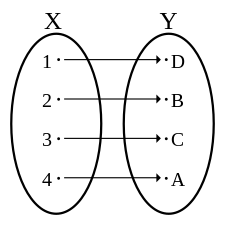
\includegraphics[height = 4.9cm]{images/bi.png}
        \caption{ TODO: ny URL her, og ny QR-kode}
        \label{fig:qrcode}
    \end{figure}
\end{frame}

%===============================================

%\section{Logikk}
\subsection{Proposisjoner}
\begin{frame}{Proposisjoner}
\begin{itemize}
    \item En proposisjon er et uttrykk med en sannhetsverdi, som alltid er enten Sann (T) elller Usann (F).
    \item Ofte setter vi dem i variabler, for å gjøre det lettere å lese.
\end{itemize}
\pause
\begin{block}{Proposisjoner}
    p := 2 < 3 \\
    q := ''Månen er laget av ost''\\
    r := ''MNF130 er et nyttig fag for informatikere''
\end{block}
\pause
\begin{block}{Ikke proposisjoner}
    ''Hva skal vi ha til middag i dag?''\\
    x + y < z
\end{block}
\end{frame}

\begin{frame}{$\lnot$, og sannhetstabeller}
\begin{itemize}
    \item Gitt en proposisjon $p$, kan vi representere den motsatte proposisjonen som $\lnot p$.
    \item Vi kan tegne opp alle mulige verdier et slikt uttrykk kan ha i en tabell.
\end{itemize}
\pause

\begin{block}{Eksempler}
    La $p := 2 < 3$. \\
    $p$ = ''Det er sant at 2 er mindre enn 3'' \\
    $\lnot p$ = ''Det er ikke sant at 2 er mindre enn 3''
\end{block}
\pause
\begin{tabular}{c|c}
$p$ & $\lnot p$ \\ \hline
T & F \\
F & T \\ \hline
\end{tabular}
\end{frame}

\begin{frame}{$\lor$ og $\land$}
    \begin{itemize}
        \item Vi kan slå sammen flere proposisjoner til et større uttrykk på mange forskjellige måter.
    \end{itemize}
    \begin{block}{Eksempel}
        La $p$ := Jorden er flat, og $q$ := Månen er flat\\
        $p \lor q$ = Jorden er flat \textbf{eller} månen er flat\\
        $p \land q$ = Jorden er flat \textbf{og} månen er flat\\
    \end{block}
    \pause
    \begin{tabular}{c|c|c|c}
        $p$ & $q$ & $p \lor q$ & $p \land q$ \\ \hline
        T & T & T & T \\
        T & F & T & F \\
        F & T & T & F \\
        F & F & F & F \\
    \end{tabular}
\end{frame}

\begin{frame}{$\rightarrow$ og $\leftrightarrow$}
    \begin{itemize}
        \item En proposisjon kan implisere en annen proposisjon.
    \end{itemize}
    \begin{block}{Eksempel}
        La $p$ := ''Det regner ute'', og $q$ := ''Bakken er våt''\\
        $p \rightarrow q$ = ''Hvis det regner ute, blir bakken våt''\\
        $p \leftrightarrow q$ = ''Det regner ute hvis og bare hvis bakken er våt''
    \end{block}
    \pause
    \begin{tabular}{c|c|c|c}
        $p$ & $q$ & $p \rightarrow q$ & $p \leftrightarrow q$ \\ \hline
        T & T & T & T \\
        T & F & F & F \\
        F & T & T & F \\
        F & F & T & T \\
    \end{tabular}
\end{frame}

\begin{frame}{Ekvivalenser og tautologier}
    \begin{itemize}
        \item Når to logiske uttrykk alltid har samme verdi, sier vi at de er \emph{logisk ekvivalente}.
        \item Om et uttrykk alltid er sant, uavhengig av innholdet, kaller vi det en tautologi.
    \end{itemize}
    \begin{tabular}{c|c|c|c}
         $p$ & $\lnot p$ & $\lnot \lnot p$ & $p \lor \lnot p$\\ \hline
         T & F & T & T\\
         F & T & F & T
    \end{tabular}
    \pause
    \begin{itemize}
        \item Konklusjon 1: $p \equiv \lnot \lnot p$
        \pause
        \item Konklusjon 2: $p \lor \lnot p \equiv T$, og er en tautologi
        \pause
        \item For å se om to uttrykk er ekvivalente, tegn sannhetstabellen og se om kollonene deres er det samme.
        \item For å se om et uttrykk er en tautologi, tegn sannhetstabellen og se om kolonnen alltid er T.
    \end{itemize}
\end{frame}

\begin{frame}{Noen viktige logiske ekvivalenser}
    \begin{columns}
    \begin{column}{0.32\textwidth}
        \begin{tabular}{l|c}
        Ekvivalens & Navn \\ \hline
        $p \land T \equiv p$ & Identity\\
        $p \lor F \equiv p$ \\ \hline
        
        $p \lor T \equiv T$ & Domination\\
        $p \land F \equiv F$\\ \hline
        
        $p \lor p \equiv p$ & Idempotent\\
        $p \land p \equiv p$ \\ \hline
        
        $p \equiv \lnot \lnot p$ & Negation\\ \hline
        
        $p \lor q \equiv q \lor p$ & Commutative\\
        $p \land q \equiv q \land p$ \\
        

    \end{tabular}
    \end{column}
    \begin{column}{0.52\textwidth}
        \begin{tabular}{l|c}
        Ekvivalens & Navn \\ \hline
        
        $(p \lor q) \lor r \equiv p \lor (q \lor r)$ & Associative\\
        $(p \land q) \land r \equiv p \land (q \land r)$ \\ \hline
        
        $p \lor (q \land r) \equiv (p \lor q) \land (p \lor r)$ & Distributive\\
        $p \land (q \lor r) \equiv (p \land q) \lor (p \land r)$ \\ \hline
        
        $\lnot (p \land q) \equiv \lnot p \lor \lnot q$ & De Morgan \\
        $\lnot (p \lor q) \equiv \lnot p \land \lnot q$ \\ \hline
        
        $p \lor (p \land q) \equiv p$ & Absorption \\
        $p \land (p \lor q) \equiv q$ \\ \hline
        
        $p \lor \lnot p \equiv T$ & Negation \\
        $p \land \lnot p \equiv F$ \\
        \end{tabular}
    \end{column}
\end{columns}
\end{frame}

\begin{frame}{Flere viktige logiske ekvivalenser}
    \begin{columns}
    \begin{column}{0.48\textwidth}
        \begin{tabular}{c}
            Ekvivalenser med $\rightarrow$ \\ \hline
            $p \rightarrow q \equiv \lnot p \lor q$ \\
            $p \rightarrow q \equiv \lnot p \rightarrow \lnot q$ \\
            $p \lor q \equiv \lnot p \rightarrow q$ \\
            $p \land q \equiv \lnot (p \rightarrow \lnot q)$ \\
            $\lnot (p \rightarrow q) \equiv p \land \lnot q$ \\
            $(p \rightarrow q) \land (p \rightarrow r) \equiv p \rightarrow (q \land r)$ \\
            $(p \rightarrow q) \land (q \rightarrow r) \equiv (p \lor q) \rightarrow r$ \\
            $(p \rightarrow q) \lor (p \rightarrow r) \equiv p \rightarrow (q \lor v)$ \\
            $(p \rightarrow r) \lor (q \rightarrow r) \equiv (p \land q) \rightarrow r$
        \end{tabular}
    \end{column}
    \begin{column}{0.48\textwidth}
        \begin{tabular}{c}
            Ekvivalenser med $\leftrightarrow$ \\ \hline
            $p \leftrightarrow q \equiv p \rightarrow q \land q \rightarrow p$ \\
            $p \leftrightarrow q \equiv \lnot p \leftrightarrow \lnot q$ \\
            $p \leftrightarrow q \equiv (p \land q) \lor (\lnot p \land \lnot q)$\\
            $\lnot (p \leftrightarrow q) \equiv p \rightarrow \lnot q$
        \end{tabular}
    \end{column}
    \end{columns}
\end{frame}

\begin{frame}{Typisk logikkoppgave}
    \begin{columns}
    \begin{column}{0.48\textwidth}
        Vis at $(p \land \lnot q) \rightarrow \lnot r$ og $(p \land r) \rightarrow q$ er logisk ekvivalente, ved å bruke enkle logiske ekvivalenser.\\[1cm]
        1. $a \rightarrow b \equiv \lnot a \lor b$ \\
        2. $\lnot (a \land b) \equiv \lnot a \lor \lnot b$\\
        3. $\lnot (\lnot a) \equiv a$
    \end{column}
    \begin{column}{0.48\textwidth}
            \pause
            $(p \land q) \rightarrow \lnot r$ \\
            \pause
            $\equiv \lnot (p \land \lnot q) \lor \lnot r$ \\
            \pause
            $\equiv (\lnot p \lor \lnot \lnot q) \lor \lnot r$ \\
            \pause
            $\equiv (\lnot p \lor q) \lor \lnot r$ \\
            \pause
            $\equiv \lnot p \lor q \lor \lnot r$ \\
            \pause
            $\equiv \lnot p \lor \lnot r \lor q$ \\
            \pause
            $\equiv \lnot (p \land r) \lor q$ \\
            \pause
            $\equiv (p \land r) \rightarrow q$
            $\qed$
    \end{column}
    \end{columns}
\end{frame}

\begin{frame}{Predikater}
    \begin{itemize}
        \item Et predikat er bare en funksjon som returnerer T eller F.
        \item Gitt et predikat og riktig antall argumenter, kan vi evaluere det som en vanlig proposisjon.
    \end{itemize}
    \begin{block}{Eksempler på predikater}
        $P(x, y, z) = x + y < z$\\
        $Q(s)$ = $s$ contains $'a'$
    \end{block}
    \pause
    \begin{block}{Eksempler på evaluering}
        $P(1, 2, 3) = 1 + 2 < 3 = 3 < 3 = F$ \\ 
        $Q($\enquote{Steinar}$) = $\enquote{Steinar} contains $'a' = T$
    \end{block}

\end{frame}

\subsection{Kvantorer}
\begin{frame}{Kvantorer (/Quantifiers)}
    \begin{itemize}
        \item Ofte vil vi si noe om et predikat $P(x)$, men for flere potensielle $x$ samtidig.
        \item $\forall x : P(x)$ = $x_1 \land x_2 \land ... \land x_n$ = ''For alle $x$ er det sant at $P(x)$''
        \item $\exists x : P(x)$ = $x_1 \lor x_2 \lor ... \lor x_n$ = ''Det eksisterer en $x$ slik at det er sant at $P(x)$''
        \item $\exists x \in S : P(x)$ = ''Det eksisterer en $x$ i settet $S$ slik at  det er sant at $P(x)$''
    \end{itemize}
    
    \pause
    \begin{block}{Eksempler}
        $\forall x : (x < x + 1)$ = ''For alle x er det sant at $x < x +1$''\\
        $\exists x : (x > x^2)$ = ''Det eksisterer en x slik at det er sant at $x > x^2$''\\
        $\exists x \in \mathbb{N} : (x*x = 1)$\\
    \end{block}
\end{frame}

\begin{frame}[fragile]{Kvantorer i praksis}
    Kvantorer ser skumle ut, men det er bare for-løkker.
    \begin{minted}[fontsize=\scriptsize]{python}
def forall(p, xs):
    for x in xs:
        if not p(x):
            return False
    return True
    
def exists(p, xs):
    for x in xs:
        if p(x):
            return True
    return False
    \end{minted}
    
    \pause
    \begin{itemize}
        \item exists(p, xs) = $\exists x \in xs : p(x)$
        \item forall(p, xs) = $\forall x \in xs : p(x)$
    \end{itemize}
\end{frame}

\begin{frame}{Nøstede kvantorer (/Nested quantifiers)}
    \begin{itemize}
        \item Ofte vil vi si noe om mange kombinasjoner av variabler samtidig.
        \item Da slår vi sammen flere $\forall$ og $\exists$.
        \item Om vi har flere like kvantorer etter hverandre kan vi slå dem sammen med tupler.
    \end{itemize}
    
    \begin{block}{Eksempler}
        $\forall x \forall y : (x^2 + y^2 \geq 0) = \forall x, y : (x^2 + y^2 \geq 0)$ \\
        $\forall x \exists y : (x * y = 1)$ = ''For alle x eksisterer det en y slik at $x * y = 1$'' \\
        $\exists x \forall y : (x^2 < y^2)$ = ''Det eksisterer en x slik at for alle y er $x^2 \leq y^2$''\\
        $\lnot \exists n, a, b, c \in \mathbb{Z} : (n > 2 \land a^n + b^n = c^n)$\\
        %$\lnot \exists n \exists a \exists b \exists c (a,b,c,n \in Z \land n > %2 \land a^n + b^n = c^n)$
    \end{block}
\end{frame}

\begin{frame}{De Morgan dukker opp igjen}
Det viser seg at De Morgan's lover også fungerer på kvantorer.\\
    \begin{columns}
    \begin{column}{0.48\textwidth}
    \begin{itemize}
        \item $\lnot \forall x : P(x)$ \\
        $\equiv \lnot [P(x_1) \land P(x_2) \land ... \land P(x_n)]$\\
        $\equiv \lnot P(x_1) \lor \lnot P(x_2) \lor ... \lor \lnot P(x_n)$\\ $\equiv \exists x : \lnot P(x)$
        \item $\lnot \exists x : P(x)$\\
        $\equiv \lnot [P(x_1) \lor P(x_2) \lor ... \lor .. P(x_n)]$\\
        $\equiv \lnot P(x_1) \land \lnot P(x_2) \land ... \land \lnot P(x_n)$\\ 
        $\equiv \forall x : \lnot P(x)$
    \end{itemize}      
    \end{column}
    \pause
    \begin{column}{0.45\textwidth}
        
\includegraphics[scale=0.3]{images/Always a bigger fish.jpeg}
        \pause
        
\includegraphics[scale=1]{images/bigger fish.PNG}
    \end{column}
    \end{columns}
\end{frame}

\subsection*{Spørretid}
\begin{frame}{Spørsmål?}
    \begin{figure}
        \centering
        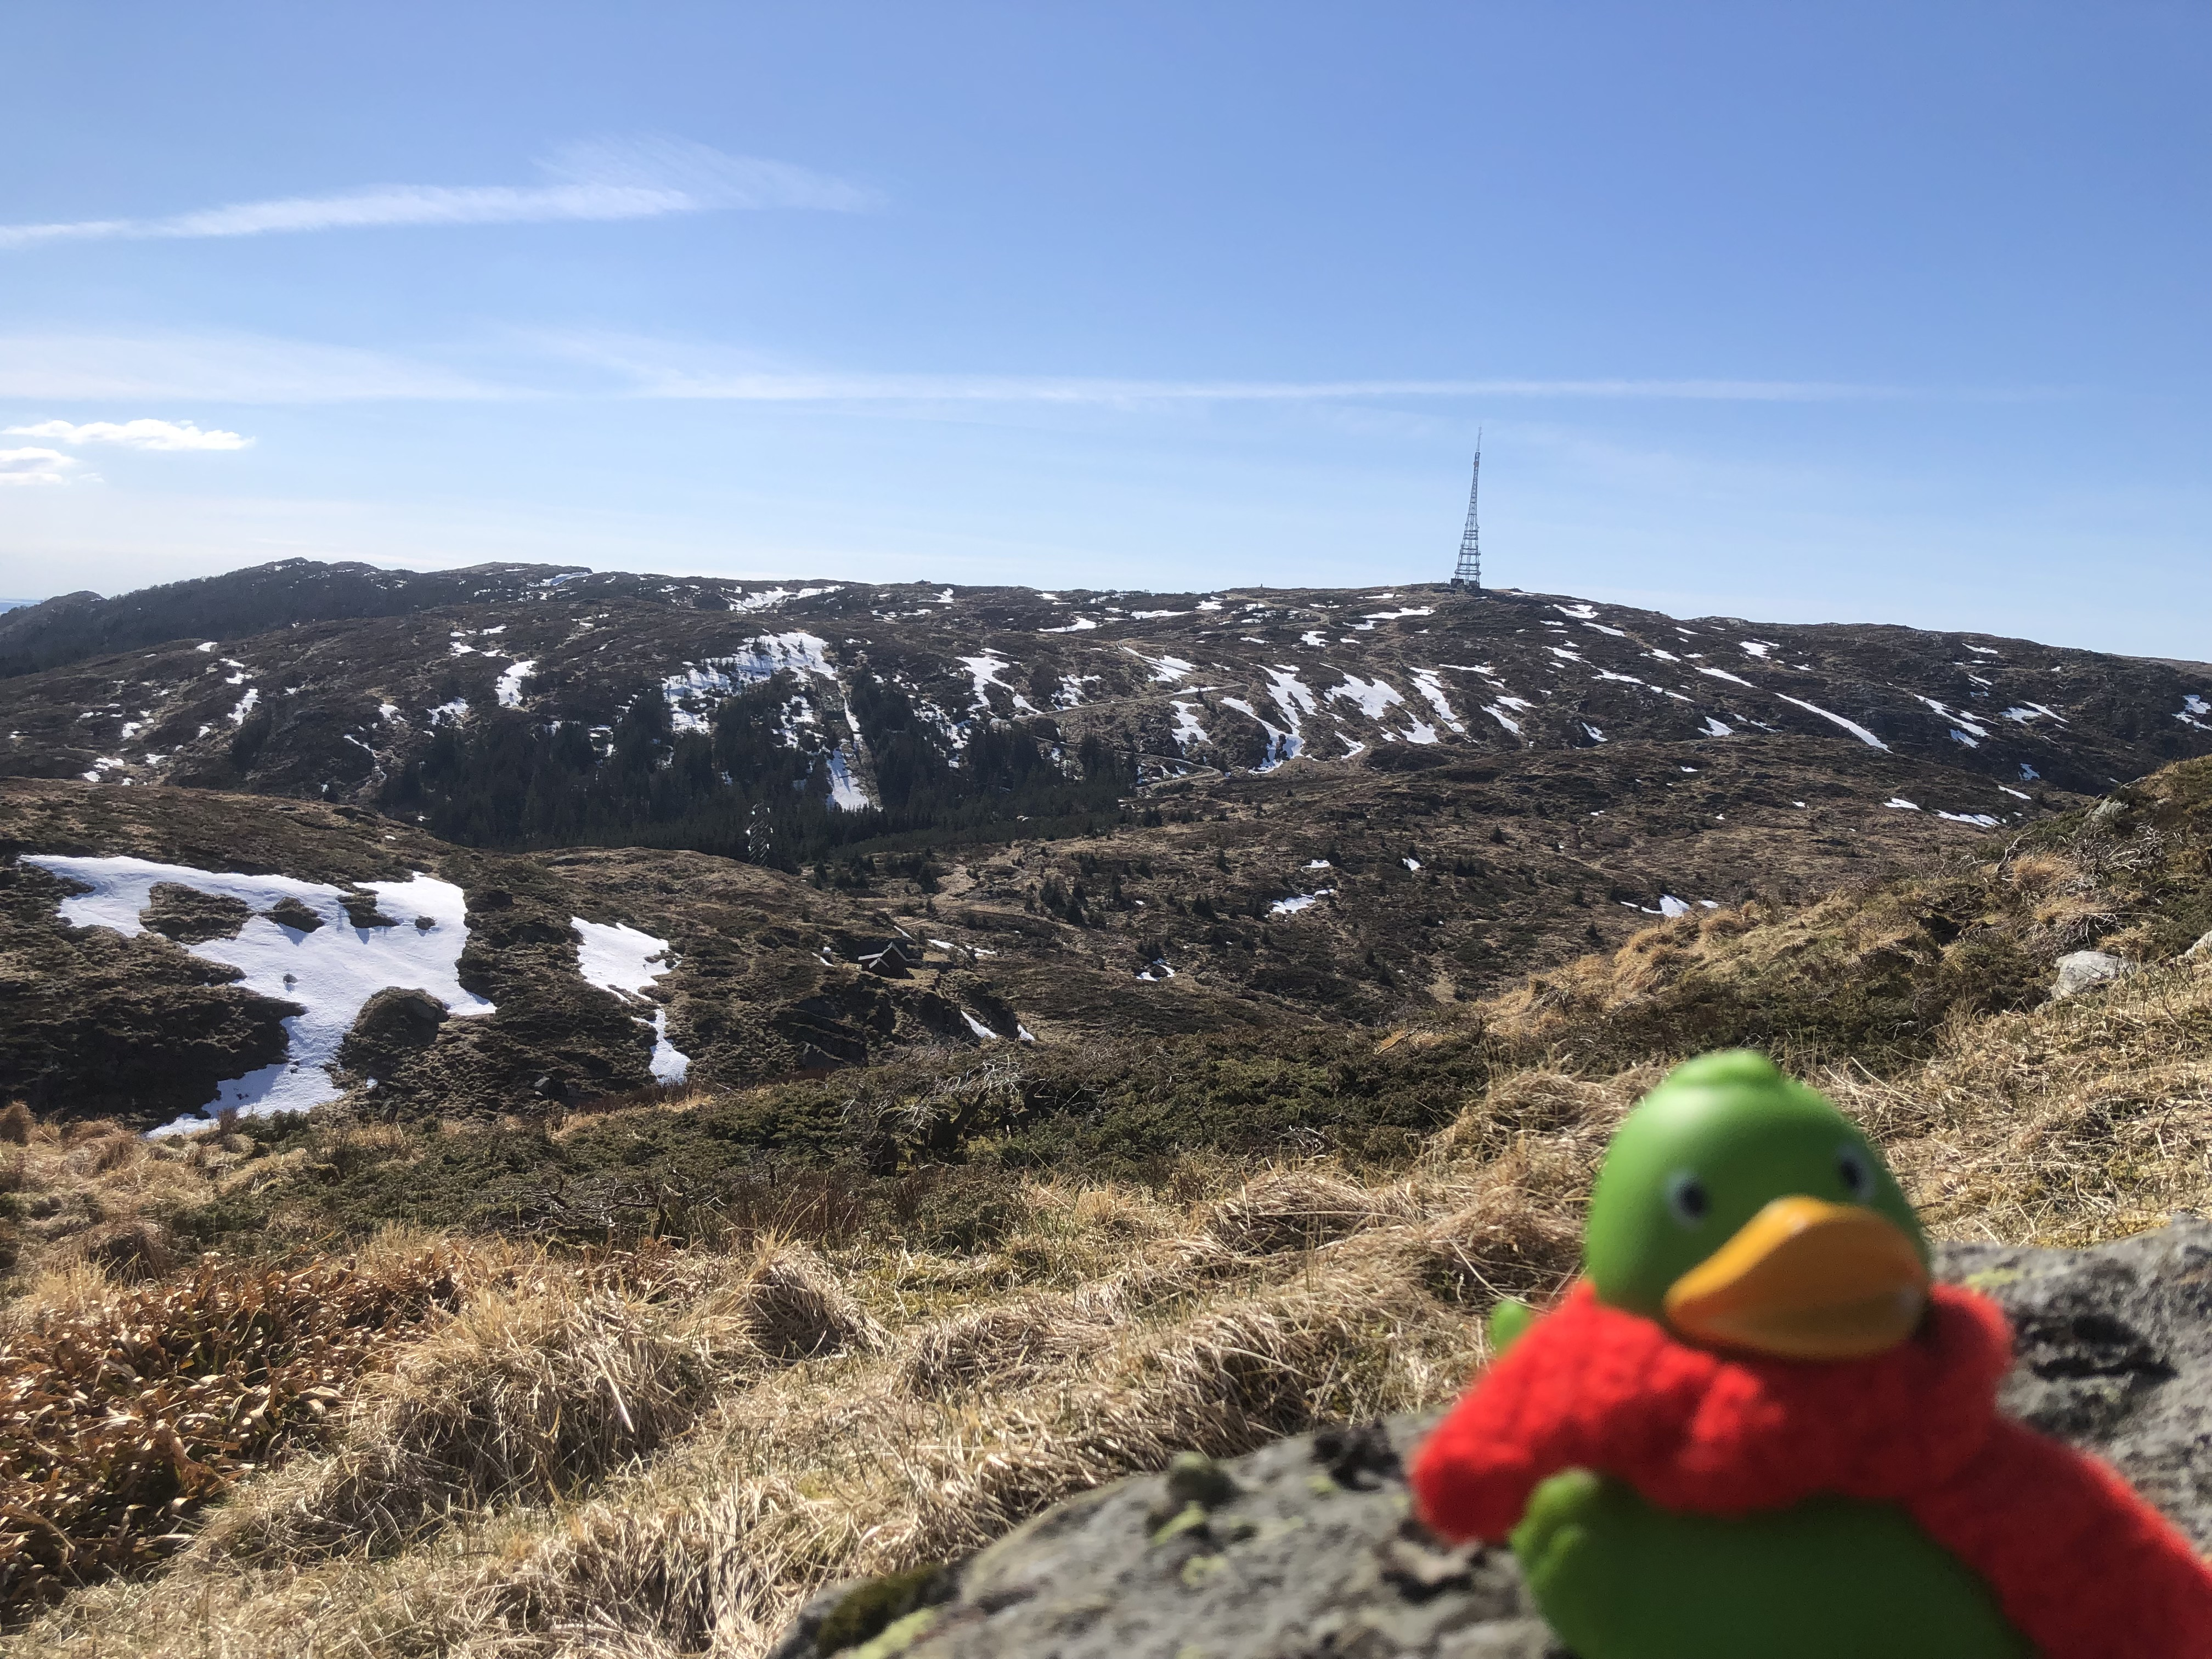
\includegraphics[height = 4.9cm]{images/guillaume5.jpg}
        \caption{Guillaume på Vidden}
        \label{fig:guillaume5}
    \end{figure}
\end{frame}
%\input{Mengdelære}
%\section{Relasjoner}
\subsection{Relasjoner}
\begin{frame}[fragile]{Relasjoner}
    En relasjon $R$ fra $A$ til $B$ er et subset av $A \times B$. De minner om funksjoner, men er et mer generelt konsept. De er lettere å visualisere ved å tegne dem:
    \begin{figure}
        \centering
        \subfloat{{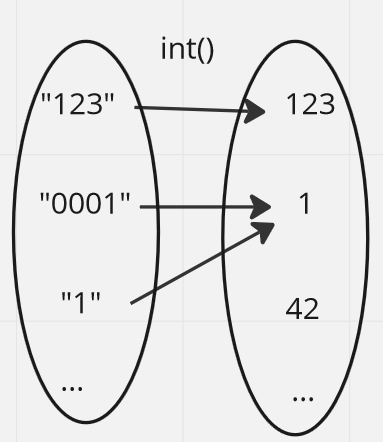
\includegraphics[width=2.8cm]{images/int again.png} }}
        \qquad
        \subfloat{{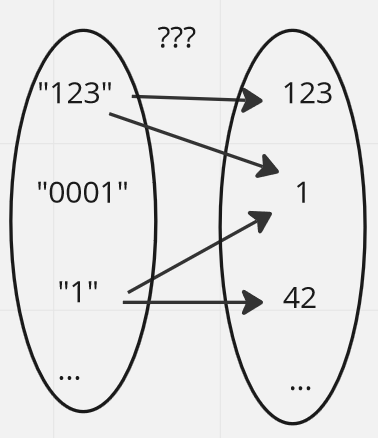
\includegraphics[width=2.8cm]{images/???.png} }}
        \qquad
        \subfloat{{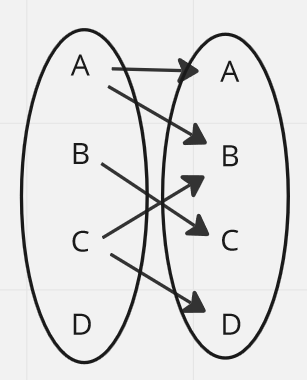
\includegraphics[width=2.8cm]{images/aa.png} }}
        \qquad
        \subfloat{{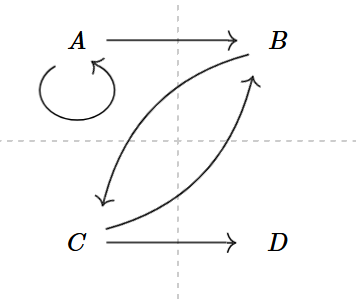
\includegraphics[width=2.8cm]{images/aaa.png} }}
        \label{fig:relasjoner}
    \end{figure} 

    \pause
    Veldig ofte er $A$ og $B$ det samme settet, dvs at $R$ er et subset av $A \times A$.\\ 
    Da kaller vi R en relasjon \emph{på} $A$.
\end{frame}

\begin{frame}[fragile]{Måter å oppgi relasjoner på}
    \begin{columns}
        \begin{column}{0.3\textwidth}
            \begin{tikzcd}
            A \arrow[r] \arrow[d] \arrow[rd] & B \arrow[d] \arrow[ld] \\
            D                                & C \arrow[l]           
            \end{tikzcd}
        \end{column}
        \begin{column}{0.65\textwidth}
            \pause
            Kantliste:\\
            $\{(A, B), (A, C), (A, D), (B, C), (B, D), (C, D)\}$\\[5mm]
            \pause
            Settkomprehensjon:\\
            $\{(x, y) | x, y \in \{A,B,C,D\}, x < y\}$:\\[5mm]
            \pause
            \begin{columns}
                \begin{column}{0.27\textwidth}
                    Matrise:\\
                    \begin{math}
                        \begin{matrix}
                              & A & B & C & D\\
                            A & 0 & 1 & 1 & 1\\
                            B & 0 & 0 & 1 & 1\\
                            C & 0 & 0 & 0 & 1\\
                            D & 0 & 0 & 0 & 0
                        \end{matrix}
                    \end{math}
                \end{column}
                \pause
                \begin{column}{0.38\textwidth}
                    Nabolister:\\        
                    $N(A) = [B, C, D]$\\
                    $N(B) = [C, D]$\\
                    $N(C) = [D]$\\
                    $N(D) = []$
                \end{column} 
            \end{columns}
        \end{column}
    \end{columns}
\end{frame}

\subsection{Egenskaper}
\begin{frame}[fragile]{Egenskaper på relasjoner}
Gitt en relasjon $R \subseteq A \times A$ på $A$ har vi 5 viktige begreper for å beskrive den:
    \begin{itemize}
        \item Refleksiv: $\forall a : ((a, a) \in R)$
        \pause
        \item Symmetrisk: $\forall a, b : [(a, b) \in R \leftrightarrow (b, a) \in R]$
        \pause
        \item Antisymmetrisk: $\forall a, b : [(a, b) \in R \land (b, a) \in R \rightarrow a = b]$
        \pause
        \item Transitiv: $\forall a, b, c : [(a, b) \in R \land (b, c) \in R \rightarrow (a, c) \in R]$\\
        \pause
        \item Om en relasjon er refleksiv, symmetrisk og transitiv, kaller vi det en ekvivalensrelasjon.
    \end{itemize}   
\end{frame}

\begin{frame}[fragile]{Refleksive relasjoner}
En relasjon $R$ er \emph{refleksiv} hvis $\forall a : ((a, a) \in R)$.\\
    \begin{columns}
        \begin{column}{0.3\textwidth}
        Ikke refleksiv:\\
        \adjustbox{scale=0.8}{
            \begin{tikzcd}
            a \arrow[dd] \arrow[rr] &  & b                                             \\
                                    &  &                                               \\
            c \arrow[rruu]          &  & d \arrow[loop, distance=2em, in=305, out=235]
            \end{tikzcd}
        }  
        \end{column}
        \pause
        \begin{column}{0.3\textwidth}
            Refleksiv:\\
            \adjustbox{scale=0.8}{
                \begin{tikzcd}
                a \arrow[dd] \arrow[rr] \arrow[loop, distance=2em, in=305, out=235] &  & b \arrow[loop, distance=2em, in=305, out=235] \\
                                                                                    &  &                                               \\
                c \arrow[rruu] \arrow[loop, distance=2em, in=305, out=235]          &  & d \arrow[loop, distance=2em, in=305, out=235]
                \end{tikzcd}
            }
        \end{column}
    \end{columns}
    \pause
    \begin{columns}
        \begin{column}{0.3\textwidth}
            \begin{math}
                \begin{matrix}
                      & a & b & c & d\\
                    a & 0 & 1 & 1 & 0\\
                    b & 0 & 0 & 0 & 0\\
                    c & 0 & 1 & 0 & 0\\
                    d & 0 & 0 & 0 & 1
                \end{matrix}
            \end{math}
        \end{column}
        \begin{column}{0.3\textwidth}
            \begin{math}
                \begin{matrix}
                      & a & b & c & d\\
                    a & 1 & 1 & 1 & 0\\
                    b & 0 & 1 & 0 & 0\\
                    c & 0 & 1 & 1 & 0\\
                    d & 0 & 0 & 0 & 1
                \end{matrix}
            \end{math}
        \end{column}
    \end{columns}
\end{frame}

\begin{frame}[fragile]{Symmetriske relasjoner}
    En relasjon $R$ er \emph{symmetrisk} hvis $\forall a, b : [(a, b) \in R \leftrightarrow (b, a) \in R]$.\\
    \begin{columns}
        \begin{column}{0.3\textwidth}
            Ikke symmetrisk:\\
            \adjustbox{scale=0.8}{
                \begin{tikzcd}
                    a \arrow[dd]   &  & b                                             \\
                                   &  &                                               \\
                    c \arrow[rruu] &  & d \arrow[loop, distance=2em, in=305, out=235]
                \end{tikzcd}
            }
        \end{column}
        \pause
        \begin{column}{0.3\textwidth}
            Symmetrisk:\\
            \adjustbox{scale=0.8}{
                \begin{tikzcd}
                    a \arrow[dd, bend left]                          &  & b \arrow[lldd, bend right]                    \\
                                                                     &  &                                               \\
                    c \arrow[rruu, bend right] \arrow[uu, bend left] &  & d \arrow[loop, distance=2em, in=305, out=235]
                \end{tikzcd}
            }
        \end{column}
    \end{columns}
    \pause
    \begin{columns}
        \begin{column}{0.3\textwidth}
            \begin{math}
                \begin{matrix}
                      & a & b & c & d\\
                    a & 0 & 0 & 1 & 0\\
                    b & 0 & 0 & 0 & 0\\
                    c & 0 & 1 & 0 & 0\\
                    d & 0 & 0 & 0 & 1
                \end{matrix}
            \end{math}
        \end{column}
        \begin{column}{0.3\textwidth}
            \begin{math}
                \begin{matrix}
                      & a & b & c & d\\
                    a & 0 & 0 & 1 & 0\\
                    b & 0 & 0 & 1 & 0\\
                    c & 1 & 1 & 0 & 0\\
                    d & 0 & 0 & 0 & 1
                \end{matrix}
            \end{math}
        \end{column}
    \end{columns}
\end{frame}

\begin{frame}[fragile]{Antisymmetriske relasjoner}
    En relasjon $R$ er \emph{antisymmetrisk} hvis $\forall a, b : [(a, b) \in R \land (b, a) \in R \rightarrow a = b]$.\\
    \begin{columns}
        \begin{column}{0.3\textwidth}
            Ikke antisymmetrisk:\\
            \adjustbox{scale=0.8}{
                \begin{tikzcd}
                a \arrow[dd, bend left]                          &  & b \arrow[lldd, bend right]                    \\
                                                                 &  &                                               \\
                c \arrow[rruu, bend right] \arrow[uu, bend left] &  & d \arrow[loop, distance=2em, in=305, out=235]
                \end{tikzcd}
            }
        \end{column}
        \pause
        \begin{column}{0.3\textwidth}
            Antisymmetrisk:\\
            \adjustbox{scale=0.8}{
                \adjustbox{scale=0.8}{
                    \begin{tikzcd}
                        a \arrow[dd]   &  & b                                             \\
                                       &  &                                               \\
                        c \arrow[rruu] &  & d \arrow[loop, distance=2em, in=305, out=235]
                    \end{tikzcd}
                }
            }
        \end{column}
    \end{columns}
    \pause
    \begin{columns}
        \begin{column}{0.3\textwidth}
            \begin{math}
                \begin{matrix}
                      & a & b & c & d\\
                    a & 0 & 0 & 1 & 0\\
                    b & 0 & 0 & 1 & 0\\
                    c & 1 & 1 & 0 & 0\\
                    d & 0 & 0 & 0 & 1
                \end{matrix}
            \end{math}
        \end{column}
        \begin{column}{0.3\textwidth}
            \begin{math}
                \begin{matrix}
                      & a & b & c & d\\
                    a & 0 & 0 & 1 & 0\\
                    b & 0 & 0 & 0 & 0\\
                    c & 0 & 1 & 0 & 0\\
                    d & 0 & 0 & 0 & 1
                \end{matrix}
            \end{math}
        \end{column}
    \end{columns}
\end{frame}

\begin{frame}[fragile]{Transitive relasjoner}
    En relasjon $R$ er \emph{transitiv} om $\forall a, b, c : [(a, b) \in R \land (b, c) \in R \rightarrow (a, c) \in R]$.\\
    \begin{columns}
        \begin{column}{0.3\textwidth}
            Ikke transitiv:
             \begin{tikzcd}
            a \arrow[r] \arrow[d] & b \arrow[d] \\
            d                     & c          
            \end{tikzcd}
        \end{column}
        \pause
        \begin{column}{0.3\textwidth}
            Transitiv:
            \begin{tikzcd}
            a \arrow[r] \arrow[d] \arrow[rd] & b \arrow[d] \\
            d                                & c          
            \end{tikzcd}
        \end{column}
    \end{columns}
\end{frame}

\begin{frame}{Relasjonskomposisjon}
    Gitt to relasjoner $R \subseteq A \times B$ og $S \subseteq B \times C$, kan vi konstruere komposisjonen $S \circ R \subseteq A \times C$:\\
    $S \circ R := \{(a, c) | (a, b) \in R \land (b, c) \in S\}$
    \pause
    \begin{figure}%
        \centering
        \subfloat{{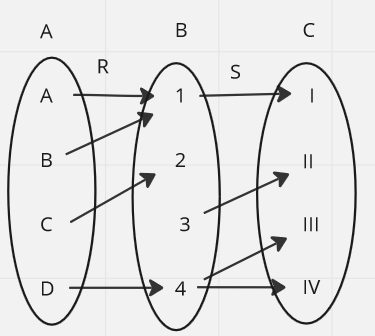
\includegraphics[width=3.3cm]{images/R, S.png} }}%
        \qquad
        \subfloat{{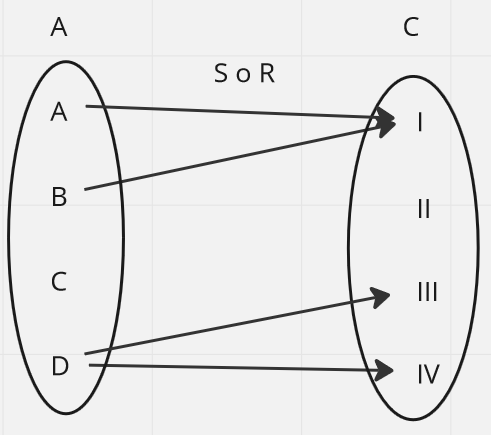
\includegraphics[width=3.3cm]{images/S o R.png} }}%
        \label{fig:ros}%
    \end{figure}
    \pause
    Obs! Som med funksjonskomposisjon er rekkefølgen er uintuitiv: R skjer før S. Dere kan lese det som $S$ 'på' $R$.
\end{frame}

\begin{frame}{Tavleoppgaver om relasjoner}
    Avgjør om følgende relasjoner er refleksive, symmetriske, anti-symmetriske, eller transitive. Er noen av dem ekvivalenserelasjoner?\\
    \begin{center}
    \begin{tabular}{ | m{15em} | m{1cm} | m{1cm} | m{1.5cm} | m{1cm} | m{1cm} | } 
      \hline
      Relasjon & Refl. & Symm. & A. Symm. & Trans. & Ekv.\\
      \hline
      $\{(a, b) | a, b \in \mathbb{N}, a < b\}$ \pause & \xmark & \xmark & \checkmark & \checkmark & \xmark \\
      \hline
      \pause
      $\{(a, b) | a, b \in \mathbb{N}, a \leq b\}$ \pause & \checkmark & \xmark & \checkmark & \checkmark & \xmark \\
      \hline
      \pause
      $B_{p, q}$ := Alle logiske uttrykk gitt av $p$ og $q$; $\{(a, b) | a, b \in B_{p, q}, a \equiv b\}$ \pause & \checkmark & \checkmark & \xmark & \checkmark & \checkmark\\
      \hline
      \pause
      $\emptyset$ \pause & \checkmark & \checkmark & \checkmark & \checkmark & \checkmark\\
      \hline
    \end{tabular}
    \end{center}
\end{frame}

\subsection*{Spørretid}
\begin{frame}{Spørsmål?}
    \begin{figure}
        \centering
        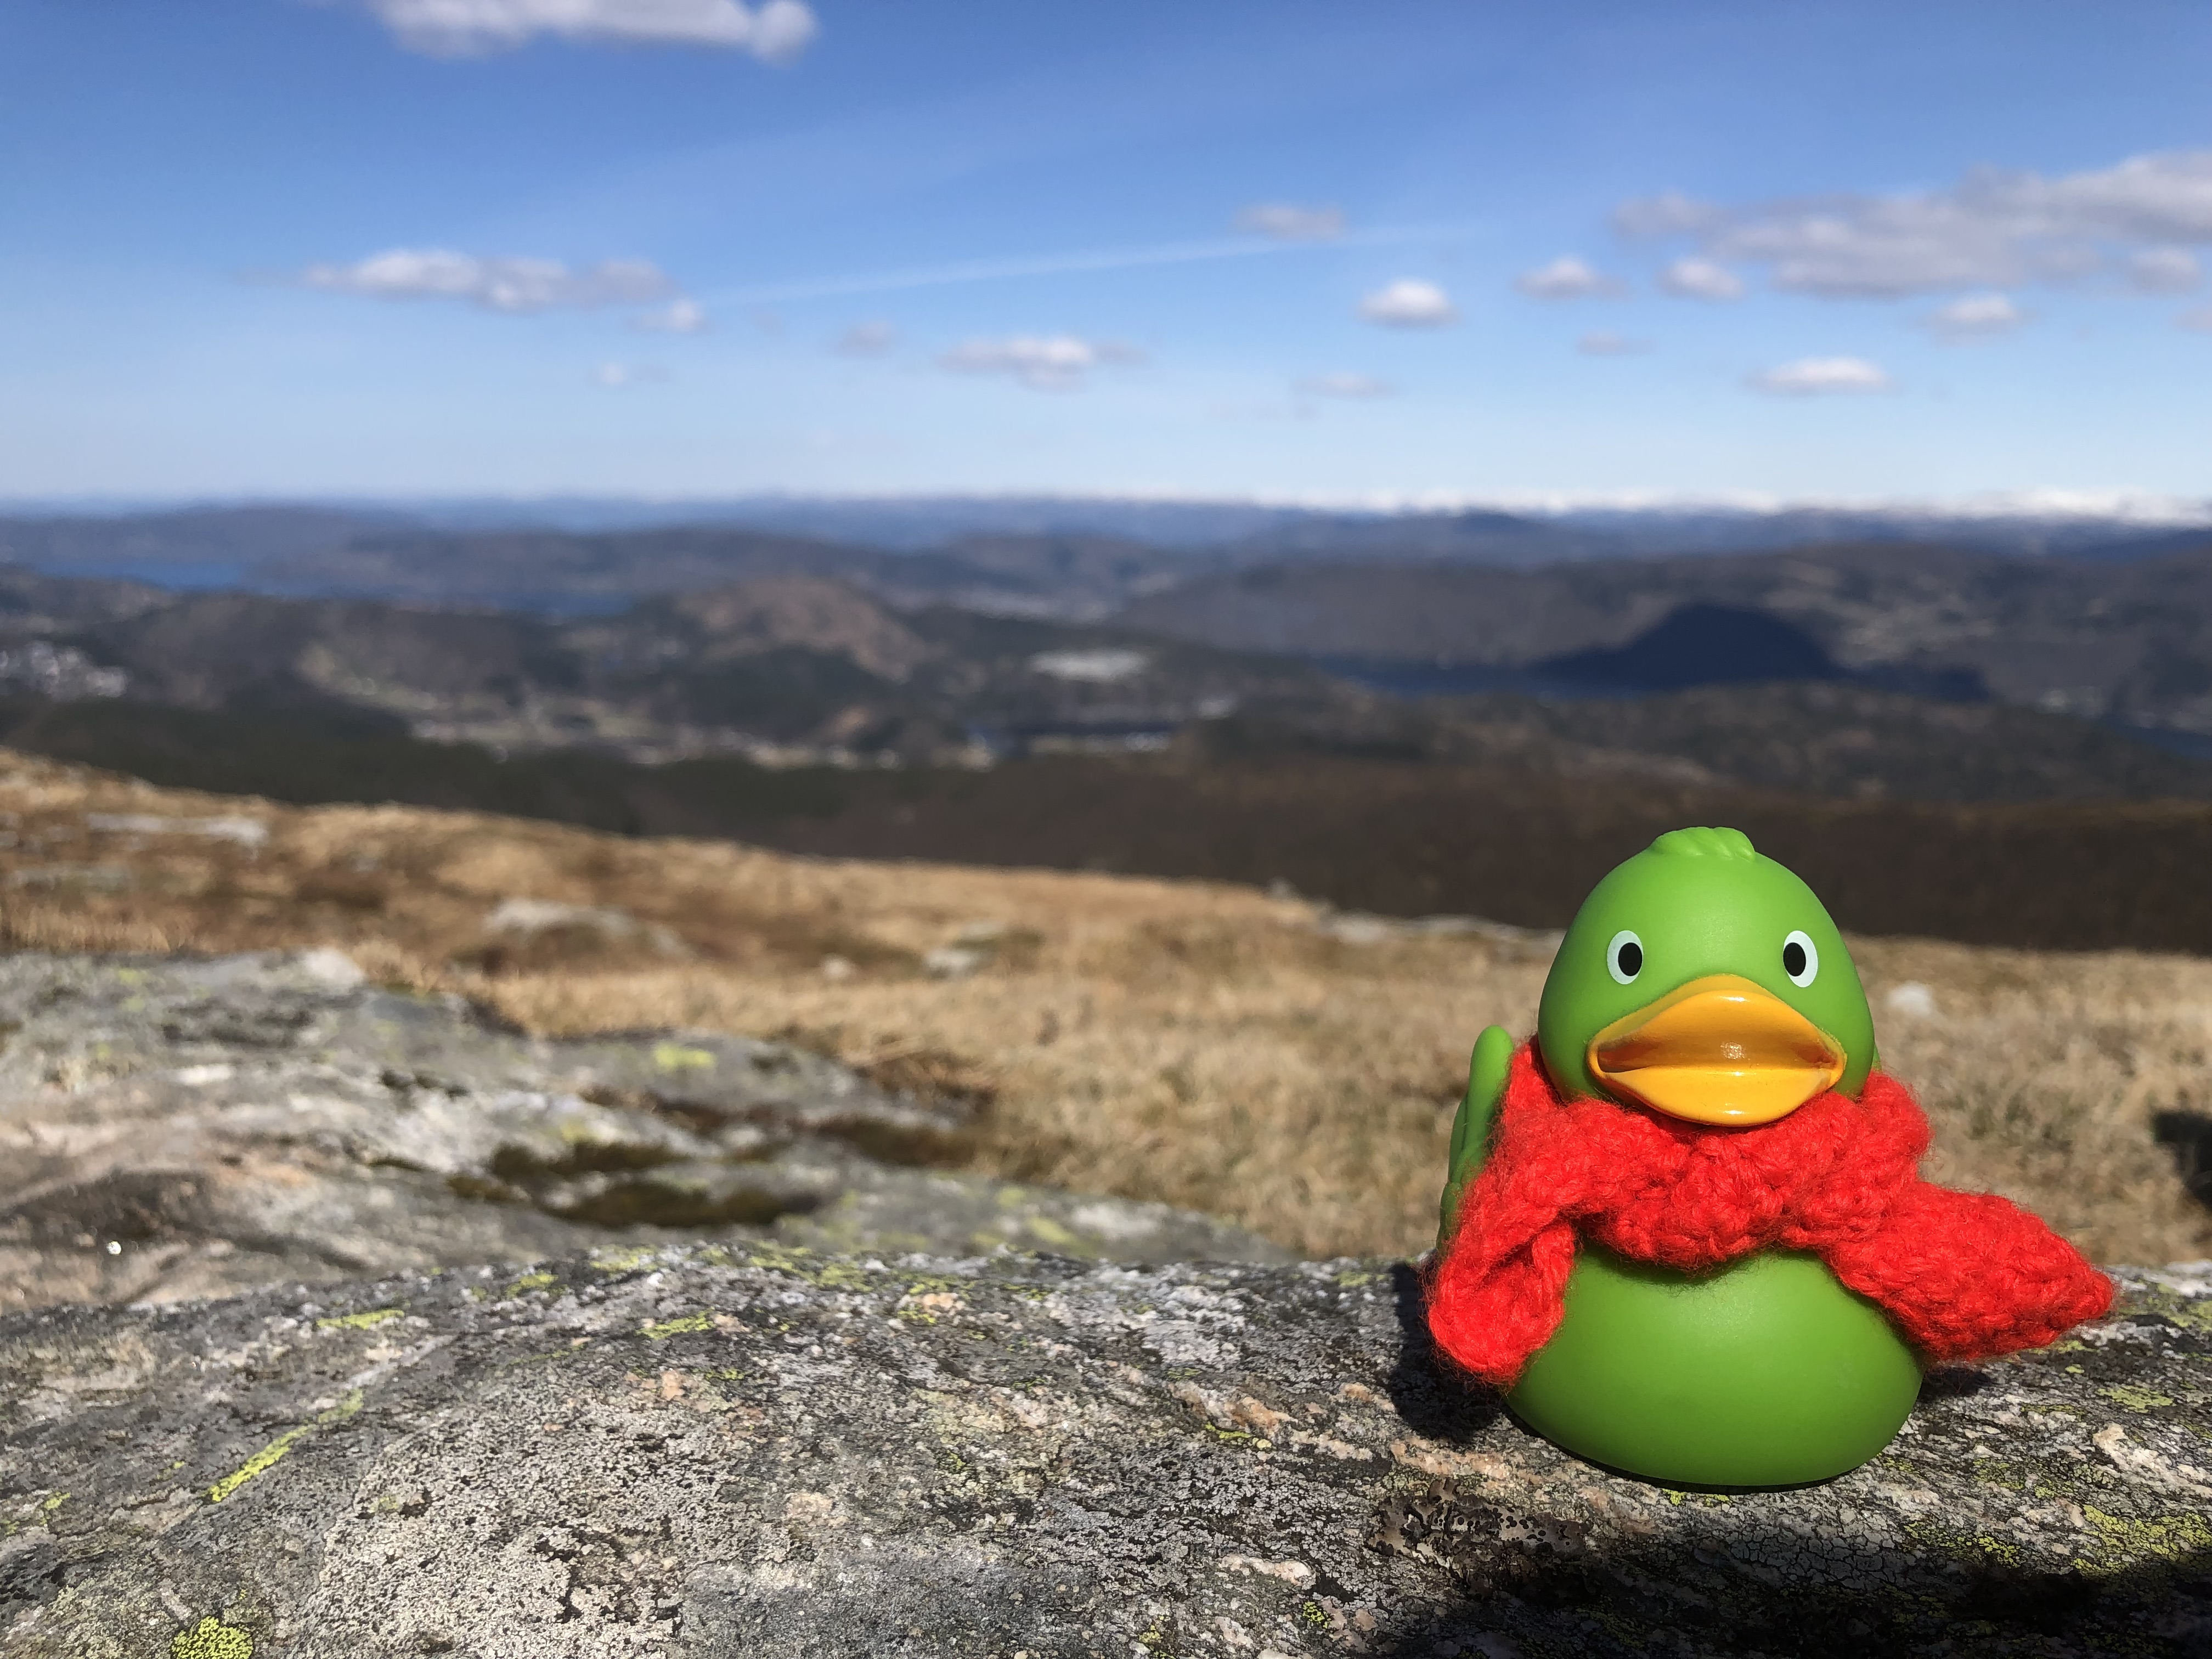
\includegraphics[height = 4.9cm]{images/guillaume3.jpg}
        \caption{Guillaume et sted Lukas ikke husker}
        \label{fig:guillaume3}
    \end{figure}
\end{frame}
%\section{Bevis}

\begin{frame}{Beviser}
    1. Hva vet vi?\\
    
    2. Hva beviser vi? \\
    
    3. Kan vi knytte det sammen?\\
    
    (4. Kan vi skriver det som formler eller kan vi tegner noe?)\\

    (5. Skrev ned hva dere prøve å bevise!) %raus?
\end{frame}

\begin{frame}{Beviser eksempel}
    %en for formler og en for tegner? Mengde? En av dem er nok?
\end{frame}

\begin{frame}{Direkte bevis}
    Et direkte bevis for $p \rightarrow q$ er et som antar at $p$ = T, og viser at det medfører at $q$ = T.\\
    Dette er ofte de enkleste bevisene. Hvis du har formler du må bare knytte sammen, forsøk det først.\\
    
    \pause
    \begin{block}{Vis at om $x$ og $y$ er oddetall, da er $x + y$ et partall.}
        Vi tar to oddetall $x$ og $y$. Da kan vi omskrive dem:\\
        $x = 2a+1$, $y = 2b+1$, for $a, b \in \mathbb{N}_0$.\\
        Nå viser vi at summen er partall: $x+y=2c$, $c \in \mathbb{N}_0$\\
        Da er $x + y = (2a+1) + (2b+1) = 2a + 2b + 2 = 2(a+b+1)$.\\
        Siden vi ganger med $2$ blir $2(a + b + 1)$ et partall uavhengig av hva $a + b + 1$ er.\\
        \qed
    \end{block}
\end{frame}

\begin{frame}{Kontrapositivt bevis (/proof by contraposition)}
    Istedet for å bevise $p \rightarrow q$, er det ofte lettere å bevise $\lnot q \rightarrow \lnot p$. De uttrykkene er helt ekvivalente.\\
    Det vil si å anta at $\lnot q = F$, og vise at da må også $\lnot p = F$.\\
    
    \pause
    \begin{block}{For ethvert heltall n har vi at hvis $n^2$ er et partall, så er n også et partall.}
        $n^2=2k \rightarrow n=2l$;    $k,l\in\mathbb{N}$\\
    \pause
        $n=2l+1 \rightarrow n^2=2k+1$\\
        $(n)^2=(2l+1)^2=4l^2+4l+1=2(2l^2+2l)+1=2k+1$ hvor $k=2l^2+2l \in\mathbb{N}$\\
    \pause
        $\implies$ hvis $n$ er IKKE et partall så er heller IKKE $n^2$ et partall.\\
        $\implies$ hvis $n^2$ er et partall så er også $n$ et partall.
        \qed
    \end{block}
\end{frame}

\begin{frame}{Motsigelsesbevis (/proof by contradiction)}
    For å bevise en proposisjon $p$, kan det vi heller bevise at $\lnot p$ leder til en motsigelse. Det vil si, motbevis det motsatte.
    
    \pause
    \begin{block}{Vis at summen av et rasjonalt tall $\frac{a}{b}$ og et irrasjonalt tall $c$ også er et irrasjonalt tall.}
    Vi antar det motsatte: at summen blir et rasjonalt tall: $\frac{a}{b}$ + $c$ = $\frac{e}{d}$ for $e, d \in \mathbb{Z}$.\\
    $\implies \frac{e}{d} - \frac{a}{b} = c$\\
    $\implies \frac{b\cdot d - a \cdot d}{b\cdot d} = c$\\
    Men det impliserer at $c$ er et rasjonalt tall. [motsigelse!]\\
    Derfor er det usant at summen er et rasjonalt tall\\
    $\implies$ summen må være irrasjonal
    \qed
    
    \end{block}
\end{frame}

\begin{frame}{Uttømmende bevis (/proof by exhaustion)}
    OBS! Ingen garanti for å få poenger! Men hvis du har tid og ikke et plan, prøv det.\\
    Noen ganger orker vi ikke finne på et elegant bevis. Da tar vi heller for oss hvert enkelt tilfelle hver for seg, og når vi har vist at det holder for alle tilfeller har vi bevist påstanden.
    \pause
    \begin{block}{Vis at alle sommer-OL har blitt arrangert i årstall delelige på 4.}
        1896 mod 4 = 0 \checkmark \\
        1900 mod 4 = 0 \checkmark \\
        1904 mod 4 = 0 \checkmark \\
        .... \\
        (de neste 24 linjene er trivielle og etterlatt som en oppgave for leseren)\\
        ....\\
        2020 mod 4 = 0 \checkmark
    \end{block}
\end{frame}

\begin{frame}{Motbeviser}
    For å bevise at en påstand er usann, holder det vanligvis bare å finne et moteksempel. Dette er vanligvis den letteste typen bevis.\\
    OBS! Det er det eneste øyeblikket hvor det er ok å stoppe etter et eksempel.
    \pause
    \begin{block}{Påstand: det er ikke mulig å plassere 8 dronninger på et sjakkbrett uten at noen av dem truer hverandre.}
    \pause
    \begin{figure}
        \centering
        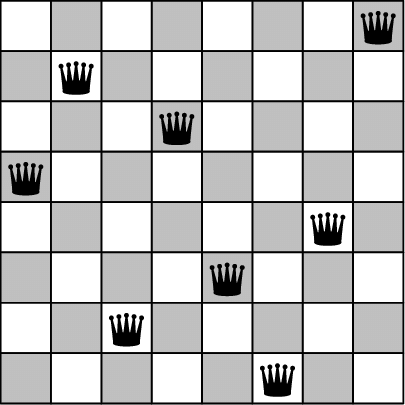
\includegraphics[scale=0.20]{images/8 queens.png}
        % \caption{Motbevis}
        \label{fig:my_label}
    \end{figure}
    
    \end{block}
\end{frame}

\subsection{Induksjon}
\begin{frame}{Matematisk induksjon}
    Et induksjonsbevis for en påstand $P(x)$ består av to steg:\\
    \begin{itemize}
        \item Vis at $P(0)$ stemmer
        \item Vis at om $P(n)$ stemmer, må $P(n+1)$ stemme
    \end{itemize}
    Dermed har vi bevist at $\forall x [ x > 0 \rightarrow P(x)]$
    
    \begin{figure}
        \centering
        
\includegraphics[scale=0.1]{images/domino.PNG}
        % \caption{}
        \label{fig:my_label1}
    \end{figure}
\end{frame}

\begin{frame}{Apen og Stigen} %bild?
    Apen stå på trinn 0.\\
    
    Hvis apen viser deg at den kan klatre opp til trinn 1, vet du om den kan klatre opp til trinn k?\\
\pause
    Nei, du vet bare at den kan klatre opp til trinn 1.\\
    
\pause
    Hvis apen viser deg at den kan klatre opp fra en vilkårlig trinn til næsten, vet du om den kan klatre opp til trinn k?\\
\pause
    Ja, vi vet at den allerede står på trinn 0 og den kan klatre fra en trinn til næste. Den kan klatre opp hver trinn.
    
\end{frame}
\begin{frame}{Eksempel på matematisk induksjon}
    Vis at $\sum_{i=0}^{n} i = \frac{n(n+1)}{2}$.\\
\pause    
    Vi lar $P(n) := \sum_{i=0}^{n} i = \frac{n(n+1)}{2}$\\%kan jeg aendre fra x til n?
    
\pause 
    Vis at $P(0)$ stemmer\\
\pause
    Vi begynner med base case, at påstanden holder for $P(0)$.\\
    $P(0): \sum_{i=0}^{0} i = \frac{0(0+1)}{2} = 0$ \checkmark\\
\end{frame}

\begin{frame}{Eksempel på matematisk induksjon (fortsettelse)}
    Vis at om $P(n)$ stemmer, må $P(n+1)$ stemme\\
    Nå antar vi at påstanden holder for $n$: \\
    $P(n): \sum_{i=0}^{n} i = \frac{n(n+1)}{2}$\\
    Nå viser vi at det medfører at påstanden også må hold for $n+1$:\\
    $P(n+1): \sum_{i=0}^{n+1} i = \frac{(n+1)((n+1)+1)}{2} = \frac{(n+1)(n+2)}{2}$\\

    $\sum_{i=0}^{n+1} i =1 + 2 + ... + n + (n+1) = (\sum_{i=0}^{n} i )+ (n+1)$\\
\pause
    med $P(n)$ $\implies \frac{n(n+1)}{2} + n + 1$\\
    $ = \frac{n(n+1)}{2}+\frac{2(n+1)}{2} = \frac{n(n+1)+2(n+1)}{2}$\\
    $ = \frac{(n+1)(n+2)}{2}$ \checkmark
\end{frame}

\begin{frame}{Sterk induksjon}
    Dette er veldig likt. Men istedet for å anta $P(k)$, antar man $P(0) \land P(1) \land .... \land P(k)$.\\
    Du kan tenke helt likt på disse to formene for induksjon, eneste forskjellen er at du kan anta litt mer i induksjonssteget.\\

    Hvis du allerede forstår induksjon, trenger du ikke definisjon for sterk induksjon. Du kan gjørde det med intuisjon.
\end{frame}

\begin{frame}{Rekursive funksjoner}
    En rekursiv funksjon er en funksjon som refererer til seg selv.
    \pause
    \begin{block}{fakultæt}
        0! := 1 \\
        n! := n * (n-1)!\\
    \end{block}    
    \pause 
    3! = 3 * 2!\\
     = 3 * 2 * 1!\\
     = 3 * 2 * 1 * 0!\\
     = 3 * 2 * 1 * 1\\
     = 6
\end{frame}

\begin{frame}{Evaluering av en rekursiv funksjon}
    $fib(0) := 0$\\
    $fib(1) := 1$\\
    $fib(n) := fib(n-1) + fib(n-2)$\\
    
    \pause
    $fib(5) = fib(3) + fib(4)$\\
    $ = [fib(1) + fib(2)] + [fib(3) + fib(2)]$\\
    $ = [1 + fib(0) + fib(1)] + [fib(2) + fib(1) + fib(1) + fib(0)]$\\
    $ = [1 + 0 + 1] + [fib(1) + fib(0) + 1 + 1 + 0]$\\
    $ = [1 + 0 + 1] + [1 + 0 + 1 + 1 + 0]$\\
    $ = 5$
\end{frame}

\begin{frame}{Rekursive definisjoner}
    Som med funksjoner kan vi også definere andre strukturer rekursivt. Med andre strukturer mener vi sett 90\% av tiden.\\
    
    De defineres med et basissteg, dvs utgangspunktet, og et rekursivt steg for å utvide det.\\
    
    \pause
    \begin{block}{Eksempel}
        Basissteg: $7 \in \mathbb{S}$.\\
        Rekursivt steg: $a \in \mathbb{S} \rightarrow 10a \in \mathbb{S}$\\
        $\mathbb{S} = \{7, 70, 700, 7000, 70000, ....\}$
    \end{block}
\end{frame}

\begin{frame}{Strukturell induksjon}
    Ofte vil vi bevise egenskaper for rekursive strukturer.\\
    Det gjøres ved to steg:\\
    \begin{itemize}
        \item Basissteget: vis at egenskap holder for strukturens basissteg.
        \item Det rekursive steget: vis at om en egenskap allerede holder for en struktur, vil en runde med rekursjon opprettholde den egenskapen.
    \end{itemize}
    
    \pause
    \begin{block}{Vis at alle tall i $\mathbb{S}$ er delelige på 7.}
        Basisteget: $\mathbb{S}$ inneholder bare $7$, og $7$ mod $7$ = 0. \checkmark\\
        Rekursive steget: Vi antar at et tall $a \in \mathbb{S}$ er delelige på 7. Så $a = 7k$, $k \in \mathbb{N}$\\
        Vi vet at også $10a \in \mathbb{S}$.\\
        $10a=10 * 7k$ så alle tall i $\mathbb{S}$ er delelige på 7.\checkmark
    \end{block}
\end{frame}

\begin{frame}{Større eksempel på strukturell induksjon}
    Basissteg: $(0, 0) \in \mathbb{T}$\\
    Rekursivt steg: $(a, b) \in \mathbb{T} \rightarrow (a+1, b) \in \mathbb{T} \land (a+1, b+1) \in \mathbb{T}$.\\
    
    Oppgave: vis at $\forall a \forall b [(a, b) \in \mathbb{T} \rightarrow a \geq b]$.\\
    
    \pause
    Basissteg: $(0, 0) \in \mathbb{T}$, og $0 \geq 0$. \checkmark\\
    Rerkursivt steg: vi antar at $\forall a \forall b [(a, b) \in \mathbb{T} \rightarrow a \geq b]$. Hvert rekursive kall legger til to nye par, $(a+1, b)$ og $(a+1, b+1)$. Vi ser på dem hver for seg:
    \begin{itemize}
        \item Om $a \geq b$ er $a+1 \geq b$.
        \item Om $a \geq b$ er $a+1 \geq b+1$. \checkmark
    \end{itemize}
    Dermed kan vi konkludere med at $\forall a \forall b [(a, b) \in \mathbb{T} \rightarrow a \geq b]$.
\end{frame}

\subsection*{Spørretid}
\begin{frame}{Spørsmål?}
    \begin{figure}
        \centering
        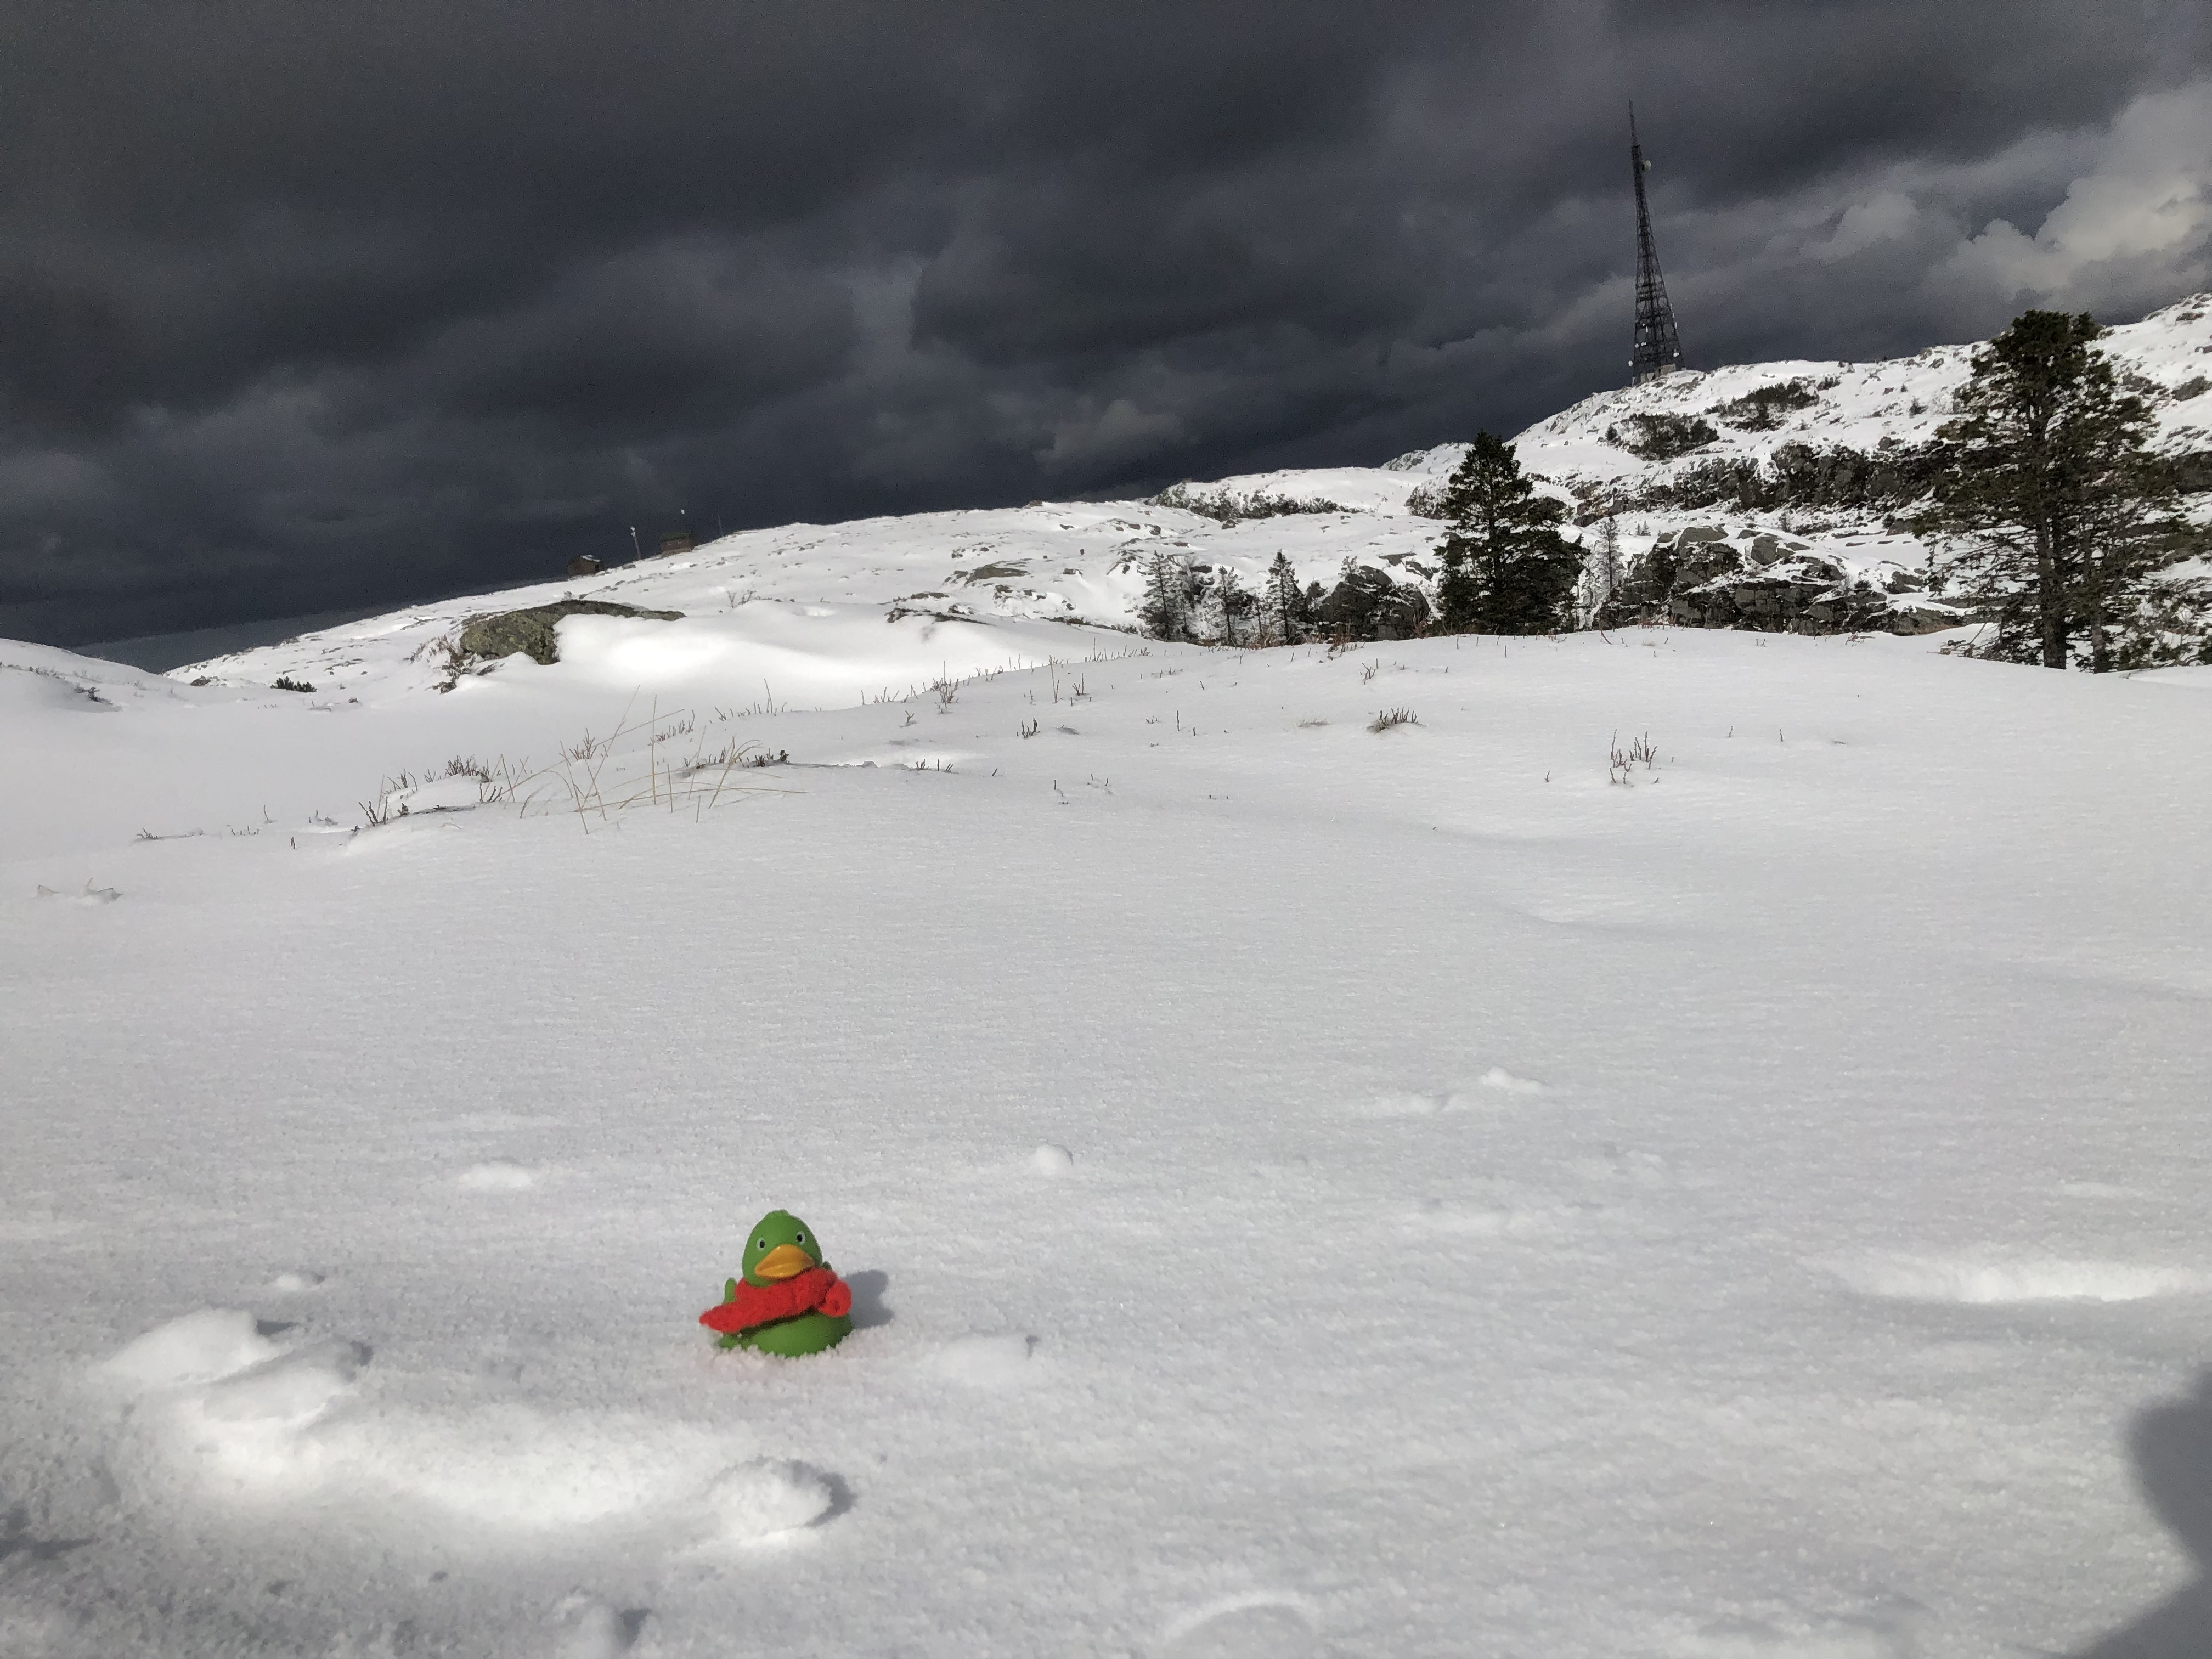
\includegraphics[height = 4.9cm]{images/guillaume7.jpg}
        \caption{Guillaume på Blåmanen}
        \label{fig:guillaume7a}
    \end{figure}
\end{frame}
%\section{Tallteori}
\subsection*{Div og mod}

\begin{frame}{Divisjon og Modulær aritmetikk}
\begin{block}{Delelighet $a|b$ ($a$ deler $b$)}
$a$ kan dele $b$ uten rest\\
$a|b$ er det samme som $\frac{b}{a}=c$ eller $b=a\cdot c$ med $c \in \matbb{Z}$\\
Eksempel: $3|12$ eller $\frac{12}{3} = 4$ eller $12=3\cdot 4$
\end{block}
\pause
\begin{block}{Modulo (Klokkearitmetikk)}
$a\, mod\, b$ gir ut resten av heltall divisjon av $\frac{a}{b}$ ($a\%b$ i programmeringsspråk)
$a\, mod\, b\, =\, r$ kalles \textit{remainder}
Eksempel: $17\, mod\, 5\, = 2$ fordi $17=3\cdot 5+2$ 
\end{block}
\end{frame}

\begin{frame}[fragile]{Algoritme for divisjon /modulo}
\begin{itemize}[<+->]
\item $d=q\cdot a + r$ med
\item $q=\floor{\frac{d}{a}}$ og $r=d\, mod\, a$
\item Eksempel: $q=\floor{\frac{17}{5}} = \floor{3.4}=3$
\item $17=3\cdot 5 + r$ $\iff$ $17=15+r$ $\iff$ $r=2$
\end{itemize}
\end{frame}

\begin{frame}{Modulo regneregler}
\begin{block}{Kongruens $\equiv$}
\begin{itemize}
\item $a \equiv b\, (mod\, m)$: a og b kongruent i forhold til mod m
\item $a \equiv b\, (mod\, m)$ betyr $a\, mod\, m=b\, mod\, m$
\item vi skriver $[a]_m := a (mod\, m)$
\item Eksempel: $8\, \equiv 3\, (mod\, 5) \equiv [3]_5$ betyr $[8]_5=3=[3]_5$ 
\end{itemize}
\end{block}
\pause
\begin{itemize}[<+->]
\item Addisjon: $[a+b]_m = [[a]_m + [b]_m]_m$
\item $[8+21]_6 = [[8]_6 + [21]_6]_6 = [2 + 3]_6 = [5]_6 = 5$
\item Multiplikasjon: $[a\cdot b]_m = [[a]_m \cdot [b]_m]_m$
\item $[8 \cdot 21]_6 = [[8]_6 \cdot [21]_6]_6 = [2 \cdot 3]_6 = [6]_6 = 0$
\end{itemize}
\end{frame}

\begin{frame}{}
\begin{exampleblock}{Eksempel}
\begin{itemize}
\item $x \equiv 3\,(mod\, 5)$ eller $[x]_5=3$
\item $y \equiv 4\,(mod\, 5)$ eller $[y]_5=4$
\item Finn løsningen: $(3\cdot x+2\cdot y^2)\, mod\,5$
\end{itemize}
\end{exampleblock}
\pause
\medskip

$[3\cdot x+2\cdot y^2]_5=[[3\cdot x]_5+[2\cdot y^2]_5]_5$\\

$[3\cdot x]_5=[[3]_5\cdot [x]_5]_5=[3\cdot 3]_5=[9]_5=4$\\
$[2\cdot y^2]_5=[[2]_5\cdot [y\cdot y]_5]_5=[[2]_5\cdot [y]_5\cdot[y]_5]_5=[2\cdot 4\cdot 4]_5=[32]_5=2$\\

$[[3\cdot x]_5+[2\cdot y^2]_5]_5=[4+2]_5=[6]_5=1$
\end{frame}

\begin{frame}[fragile]{Modulo subtraksjon og divisjon}
       Vi vet at vi har addisjon og multiplikasjon, men hva er med subtrasjon og divisjon?\\

Substraksjon:\\
$[6-3]_8=[3]_8$\\
$[3-6]_8$?\\
\pause
$[3-6]_8=[-3]_8=[0-3]_8=[8-3]_8=[5]_8=5$\\

Subtraksjon fungerer også for modulo.  
\end{frame}

\begin{frame}{Modulo subtraksjon og divisjon}
Vi vet at vi har addisjon og multiplikasjon, men hva med subtrasjon og divisjon?\\

Divisjon:\\
$[6/3]_8=[2]_8$? \pause ja, fordi $[2\cdot 3]_8=[6]_8$\\
$[3/6]_8$?\\
\pause
Nei, noen ganger fungerer det, noen ganger fungerer det ikke.\\

Vi kan ikke alltid dele!
\end{frame}

\subsection*{Tallsystem}
\begin{frame}
\begin{block}{Tallsystem}
En representasjon av tall med forskjellige tegn med en base
\end{block}
\pause

\medskip

\begin{table}[]
\centering
\label{tab:tallsystemer}
\begin{tabular}{l|l|l|l|l}
Navn & Sifre & 5 & 11 & 34 \\ \hline
Desimal (b=10) & 0-9 & 5& 11 & 34 \\
Binær (b=2) & 0-1 & 101 & 1011 & 100010 \\
Octal (b=8) & 0-7 & 5&  13 & 42\\
Hexadesimal (b=16) & 0-9,a-f& 5& B& 22\\
base=13 & 0-9,a-c & 5& B& 28
\end{tabular}
\caption{Eksempler på forskjellige tallsystemer}
\end{table}
\end{frame}

\subsection*{Konvertering av tallsystem}
\begin{frame}[fragile]{Desimal til base b}
\begin{columns}
    \begin{column}{0.30\textwidth}
    \begin{block}{pseudokode}
            tall n til base b:\\
            next digit = $n\%b$\\
            $n=\floor{\frac{n}{b}}$\\
            forsette med det til $n=0$
    \end{block}
    \end{column}
 	\pause
    \begin{column}{0.66\textwidth}
\begin{table}
\begin{tabular}{r|c|r}
n & nextDigit & output \\ \hline
22 & & 0 \\
11 & 0 & 0\\
5 & 1 & 10\\
2 & 1 & 110\\
1 & 0 & 0110\\
0 & 1 & 10110
\end{tabular}
\caption{Eksempel for dec til base 2}
\end{table}
 	\end{column}
 	\end{columns}
\end{frame}

\begin{frame}[fragile]{Base b til desimal}
\begin{columns}
    \begin{column}{0.30\textwidth}
\begin{block}{pseudokode}
    tall n og base b\\
    $sum=0$; $index=0$\\
    starter med først siffer $s$:\\
    $sum+=base^{index}\cdot s$\\
    $index+=1$\\
    forsette med hver siffer $s$
\end{block}
 	\end{column}
 	\pause
    \begin{column}{0.66\textwidth}
\begin{table}
%\begin{tabular}{r|r|r}
%toAdd & n & sum \\ \hline
% & 10110 & 0\\
%0 & 1011 & 0\\
%2 & 101 & 2\\
%4 & 10 & 6\\
%0 & 1 & 6\\
%16 & 0 & 22
%\end{tabular}
\begin{tabular}{c|r|r|r|r|r}
    tall & 1 & 0 & 1 & 1 & 0 \\ \hline
    base & 16 & 8 & 4 & 2 & 1 \\ \hline
    produkt & 16 & 0 & 4 & 2 & 0 
\end{tabular}
\caption{Eksempel for 2 til dec}
\end{table}
\begin{center}
$16+0+4+2+0=22$    
\end{center}

 	\end{column}
 	\end{columns}
\end{frame}

\subsection*{Primtall, Greatest common divisor, Least common multiple}
\begin{frame}
\begin{block}{Primtall}
Et tall som bare kan deles av seg selv og 1\\
Eksempler: 2,3,5,7,11,13,...
\end{block}
\pause
\begin{block}{Største felles faktor (/Greatest common divisor)}
$gcd(a,b) := $det største tallet som deler både a og b\\
Eksempel: $gcd(4,6)=2$\\
Co-prime: a og b er co-prime dersom $gcd(a,b)=1$
\end{block}
\pause
\begin{block}{Laveste felles multiplum (/Least common multiple)}
$lcm(a,b) := $ det minste tallet som kan deles av både a og b\\
Eksempel: $lcm(4,6)=12$\\
hvis $a\cdot b=gcd(a,b)\cdot lcm(a,b)$\\
$gcd(a,b) = 1$ $\rightarrow lcm(a,b) = a\cdot b$
\end{block}
\end{frame}

\subsection*{Euklids algoritme}
\begin{frame}[fragile]{Euklids algoritme}
\begin{columns}
    \begin{column}{0.45\textwidth}
\begin{minted}[fontsize=\scriptsize]{python}
def gcd(a, b):
    while b != 0:
        r = a % b
        a = b
        b = r
    return a
\end{minted}
 	\end{column}
 	\pause
    \begin{column}{0.45\textwidth}
    \begin{center}
       gcd(28,12)\\
       
    $28=2\cdot 12+4$\\
    $12=3\cdot 4+0$\\
    
    gcd(28,12)=4 
    \end{center}
 	\end{column}
\end{columns}


\end{frame}

\begin{frame}[fragile]{}
\begin{block}{Utvidet Euklids algoritme}
Regner ut to parameter $s$ og $t$ slik at $gcd(a,b)$ kan skrives som linærkombinasjon\\
$gcd(a,b)=s\cdot a+t\cdot b$\\
$gcd(12,28)=4=-2\cdot 12 + 1\cdot 28$\medskip

Kan brukes for å finne multiplikativt invers\\
Multiplikativ inverse finnes dersom $gcd(a,b)=1$
\end{block}
\pause

\begin{block}{Finne multiplikativt invers for $a$ med $mod\, m$}
\begin{itemize}
\item Funker bare dersom $gcd(a,m)=1$\\
\item Regn ut linærkombinasjon $gcd(a,b)=s\cdot a+t\cdot b$ med gcd
\item $a\cdot x \equiv 1 (mod\, m)$ er multiplicative inverse
\end{itemize}
\end{block}
\end{frame}

\begin{frame}{Extended Euklids algoritme}
    \begin{columns}
        \begin{column}{0.45\textwidth}
             gcd(26,7)\\
             
             $(26)=3\cdot (7)+(5)$\\
             $(7)=1\cdot (5)+(2)$\\
             $(5)=2\cdot(2)+(1)$\\
             $(2)=2\cdot(1)+(0)$\\
             
             gcd(26,7)=1
        \end{column}
        \pause
        \begin{column}{0.45\textwidth}
            Nå går vi tilbake:\\
            $(5)=2\cdot(2)+1$\\
            
            $\implies 1=(5)-2\cdot (2)$\\
            $=(5)-2\cdot ((7)-(5))$\\
            $=3\cdot (5)-2\cdot(7)$\\
            $=3\cdot ((26)-3\cdot (7))-2\cdot (7)$\\
            $=3\cdot (26)-11\cdot (7)$
        \end{column}
    \end{columns}
\end{frame}


\begin{frame}{Eksempel Multiplikativt Invers}
\begin{itemize}[<+->]
\item Hva er multiplikativt invers av $7\, mod\, 26$? ($a\cdot 7=1\, mod\, 26$)
\item $gcd(a,m) = gcd(7,26)=1$ $\rightarrow$ har multiplikativt invers
\item Linærkombinasjon fra gcd: $3\cdot (26)-11\cdot (7)=1$
\item $[1]_{26}=[3\cdot (26)-11\cdot (7)]_{26}=[-11\cdot 7]_{26}$
\item $a=-11$
\item $[-11]_{26}=[26-11]_{26}=[15]_{26}=15$
\item 15 er inverse av 7 modulo 26

\end{itemize}
\end{frame}

\subsection*{Spørretid}
\begin{frame}{Spørsmål?}
    \begin{figure}
        \centering
        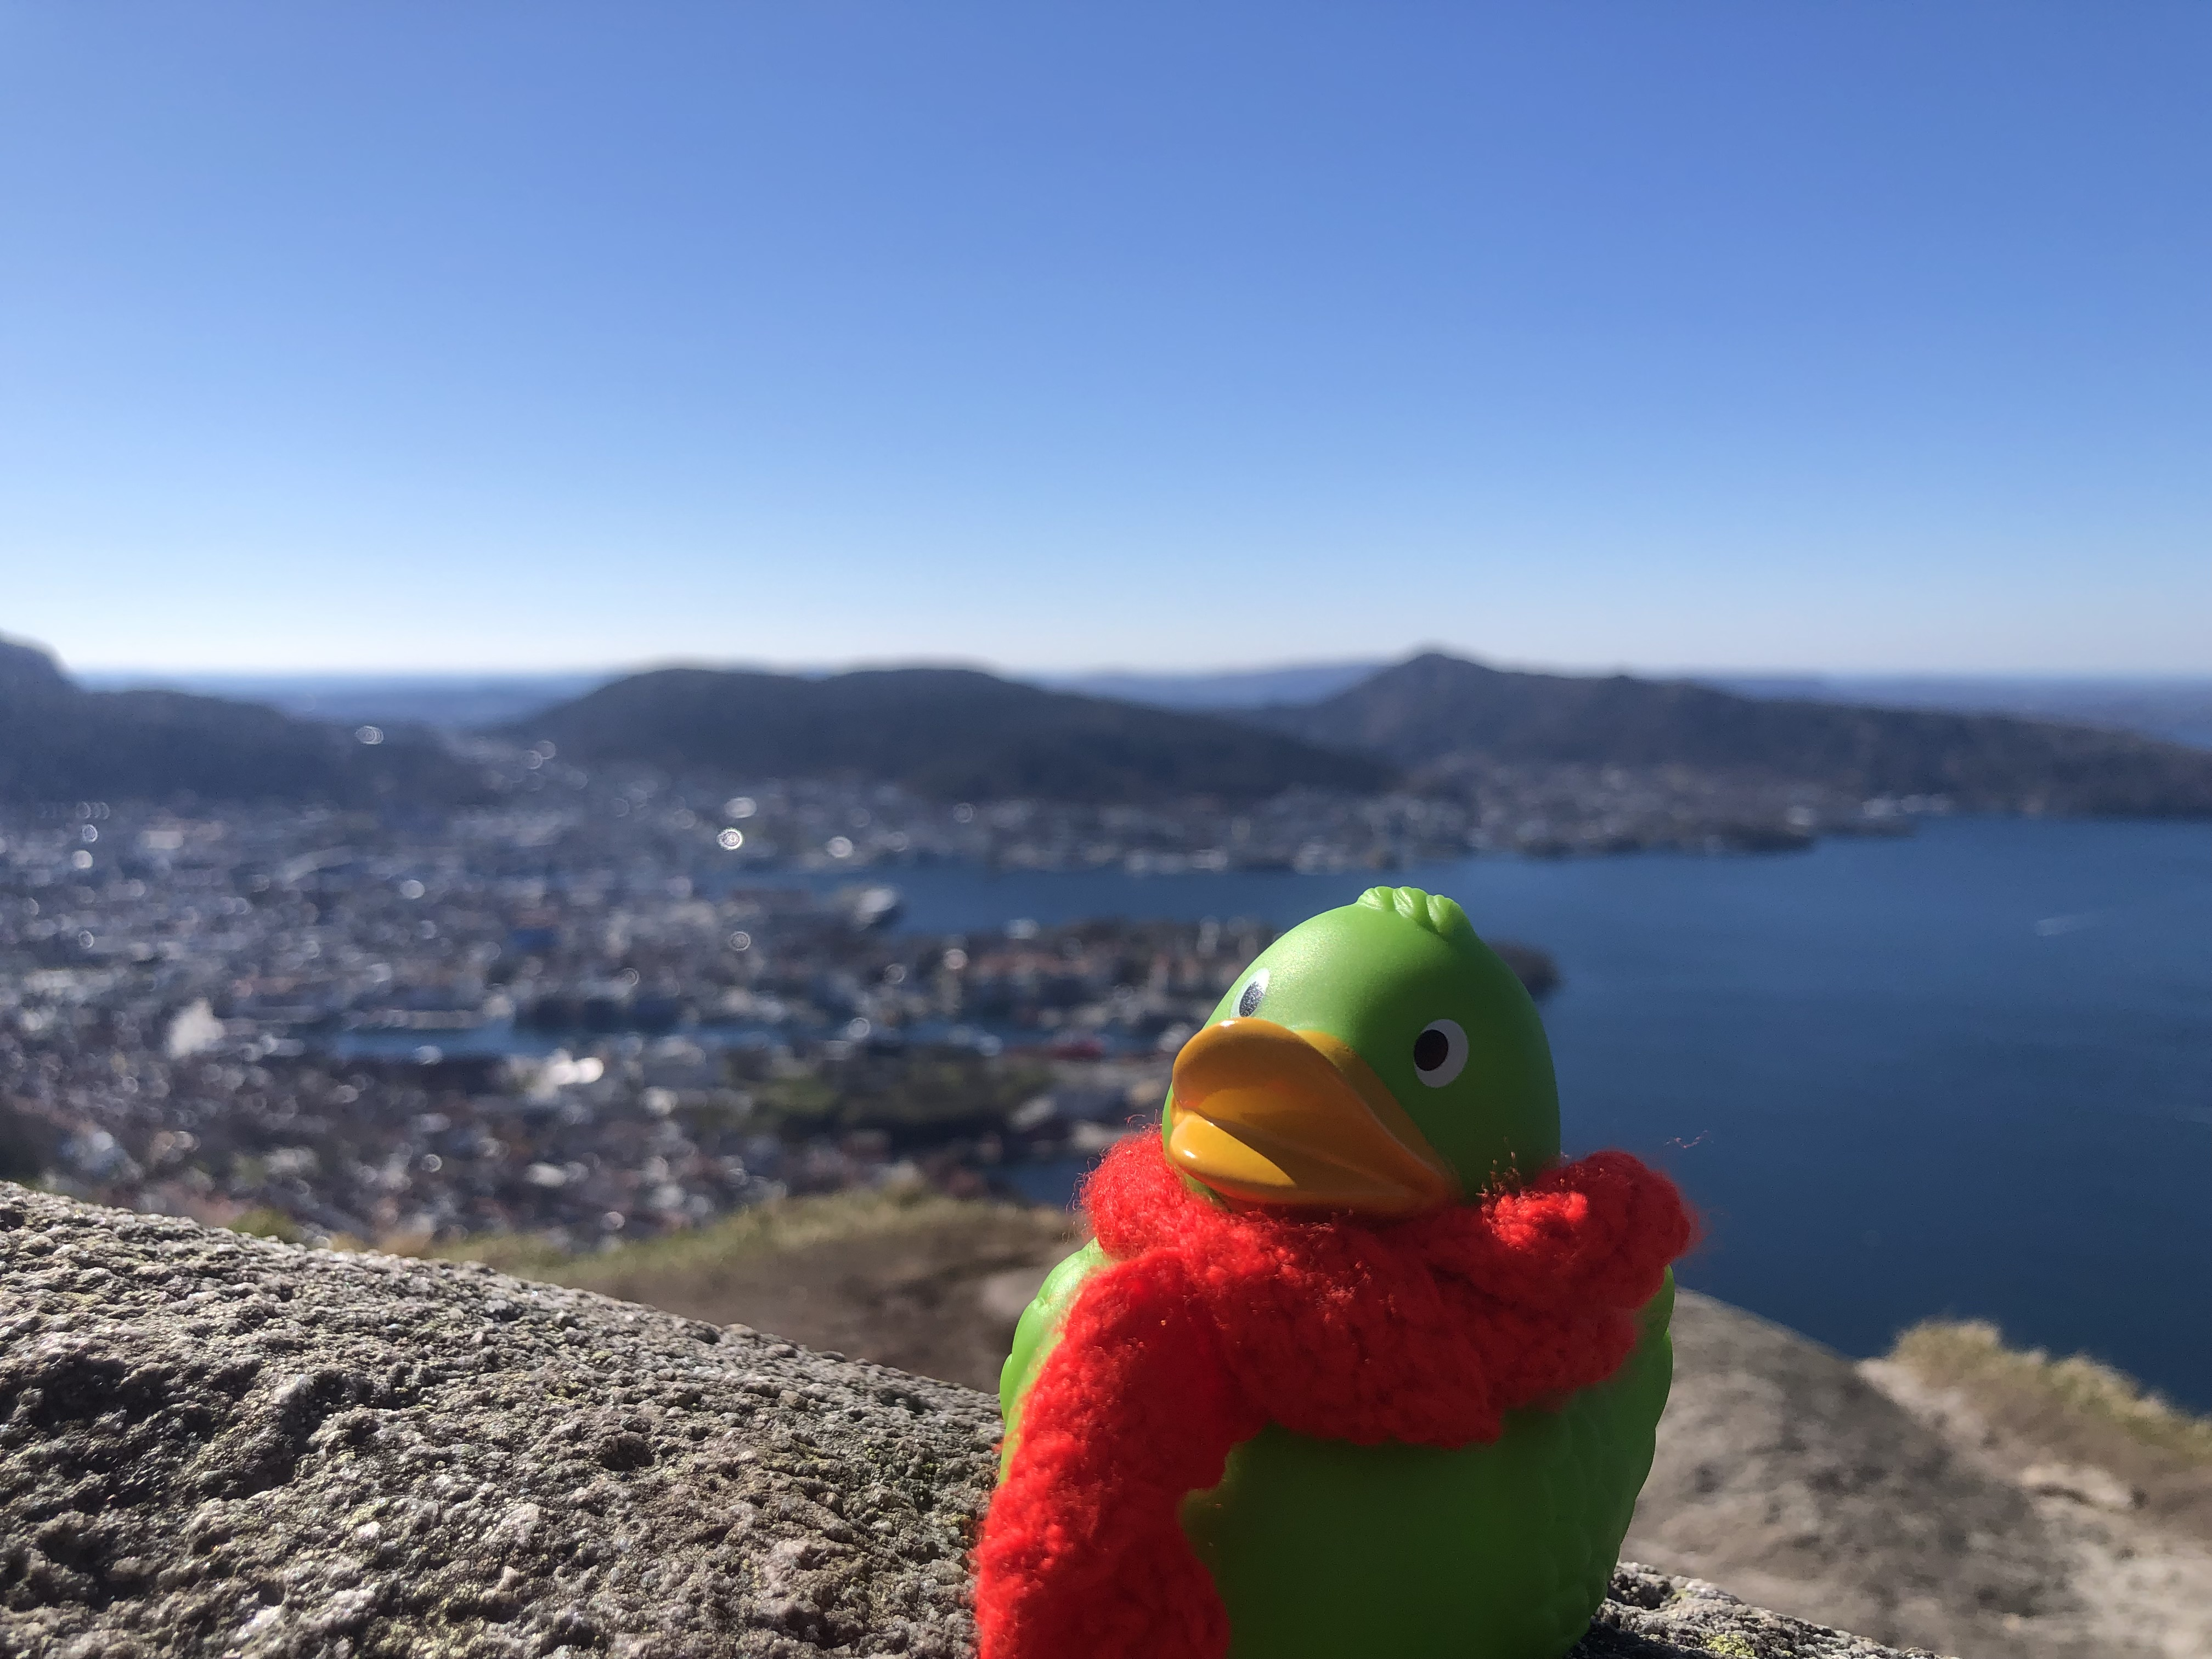
\includegraphics[height = 4.9cm]{images/guillaume1.jpg}
        \caption{Guillaume på Sandviksfjellet}
        \label{fig:guillaume1}
    \end{figure}
\end{frame}

% ===========================

\section{Kryptografi}
\subsection*{Begrep}
\begin{frame}{Symmetrisk og asymmetrisk kryptografi}
\begin{block}{Symmetrisk kryptografi}
\begin{itemize}
\item Det finnes bare \textit{én} nøkkel, som begge personer bruker
\item Brukes for både kryptering og dekryptering
\end{itemize}
\end{block}
\pause
\begin{block}{Asymmetrisk kryptografi}
\begin{itemize}
\item Hver person har \textit{to} nøkler: Privat og offentlig
\item Kryptering med offentlig nøkkel av den andre personen
\item Dekryptering med privat nøkkel
\item Eksempel: RSA
\end{itemize}
\end{block}
\end{frame}

\begin{frame}{Symmetrisk kryptografi}
    $f(c)=[c+key]_{26}$\\
    med $key=2$\\
    $f(ZEBRA)=BGDTC$\\
    
    $f^{-1}(d)=[d-key]_{26}$\\
    $f^{-1}(BGDTC)=ZEBRA$
\end{frame}

\subsection*{RSA}
\begin{frame}{RSA}
\begin{itemize}[<+->]
\item Asymmetrisk kryptering med to nøkler for hver deltaker
\item Kryptering
	\begin{itemize}
	\item Offentlig nøkkel for kryptering (n,e)
	\item Privat nøkkel for dekryptering d
	\end{itemize}
 \item $d$ er inverset av $e$ modulo $(p-1)\cdot (q-1)$ 
 \item med $p\cdot q=n$ og p,q er primtall
\end{itemize}
\end{frame}

\begin{frame}{}
    \begin{columns}
        \begin{column}{0.45 \textwidth}
            Instruksjon:\\
            velg to primtall $p,q$\\
            $n=p\cdot q$
            Velg $e$ med $2<e<\phi(n)=(p-1)\cdot (q-1)$ og $gcd(e,\phi(n))=1$\\
            Finn $d=[e^{-1}]_{\phi(n)}$\\
            Gir ut bare offentlig nøkkel $(n,e)$
        \end{column}
        \begin{column}{0.45 \textwidth}
            Eksempel:\\
            $p=7,\,q=13$\\
            $n=7\cdot 13=91$\\
            $e$ mellom $2$ og $6\cdot 12=72$ og $gcd(e,72)=1$\\
            Vi prøve 23 på neste slide:
        \end{column}
    \end{columns}
\end{frame}

\begin{frame}{Finn $d$ og $e$}
    \begin{columns}
        \begin{column}{0.45 \textwidth}
            $gcd(72,23):$\\
            $(72)=3\cdot (23)+(3)$\\
            $(23)=7\cdot(3)+(2)$\\
            $(3)=1\cdot (2)+(1)$\\
            $(2)=2\cdot (1)+(0)$\\
            gcd(72,23)=1\\
            Vi har $e=23$
        \end{column}
        \begin{column}{0.45 \textwidth}
            Når finner vi $d=[e^{-1}]_{72}$:\\
            $1=(3)-1\cdot (2)$\\
            $=(3)-((23)-7\cdot (3))$\\
            $=8\cdot (3)-(23)$\\
            $=8\cdot ((72)-3\cdot (23))-(23)$\\
            $=8\cdot (72)-25\cdot (23)$\\
            $\implies d=[-25]_{72}=[72-25]_{72}=47$
        \end{column}
    \end{columns}
\end{frame}

\begin{frame}{Kryptering}
    \begin{column}{0.45 \textwidth}
        Kryptering av blokk M:\\
        $C=[M^{e}]_{n}$\\
        $M=42$; $n=91, e=23$\\
        men $42^{23}=2.16\times 10^{37}$\\
        \pause
        $e=23=10111_2$\\
        
        $[42^{23}]_{91}=[42^{1}]_{91}\cdot[42^{2}]_{91}\cdot[42^{4}]_{91}\cdot [42^{16}]_{91}$
        \end{column}
        \pause
        \begin{column}{0.45 \textwidth}
         $[42^1]_{91}=42$\\
         $[42^2]_{91}=[1764]_{91}=35$\\
         $[42^4]_{91}=[35^2]_{91}=[1225]_{91}=42$\\
         $[42^8]_{91}=[42^2]_{91}=35$\\
         $[42^{16}]_{91}=[35^2]_{91}=42$\\
         
         $[42^{23}]_{91}=[42\cdot 35\cdot 42\cdot 42]_{91}=[2593080]_{91}=35$
        \end{column}
\end{frame}

\begin{frame}{Dekryptering}
    \begin{columns}
        \begin{column}{0.45 \textwidth}
        Dekryptering av blokk C:\\
        $M=[C^d]_{n}$\\
        $C=35$; $n=91, d=47$\\
        $d=47=101111_2$\\
        \end{column}

        \begin{column}{0.45 \textwidth}
        $[35^1]_{91}=35$\\
        $[35^2]_{91}=42$\\
        $[35^4]_{91}=35$\\
        $[35^8]_{91}=42$\\
        $[35^{16}]_{91}=35$\\
        $[35^{32}]_{91}=42$\\
        $[35^{47}]_{91}=[35\cdot 42\cdot 35 \cdot 42 \cdot 42]_{91}=[35^2\cdot 42^3]_{91}=[42^4]_{91}=42$
        \end{column}
    \end{columns}
\end{frame}

\subsection*{Spørretid}
\begin{frame}{Spørsmål?}
    \begin{figure}
        \centering
        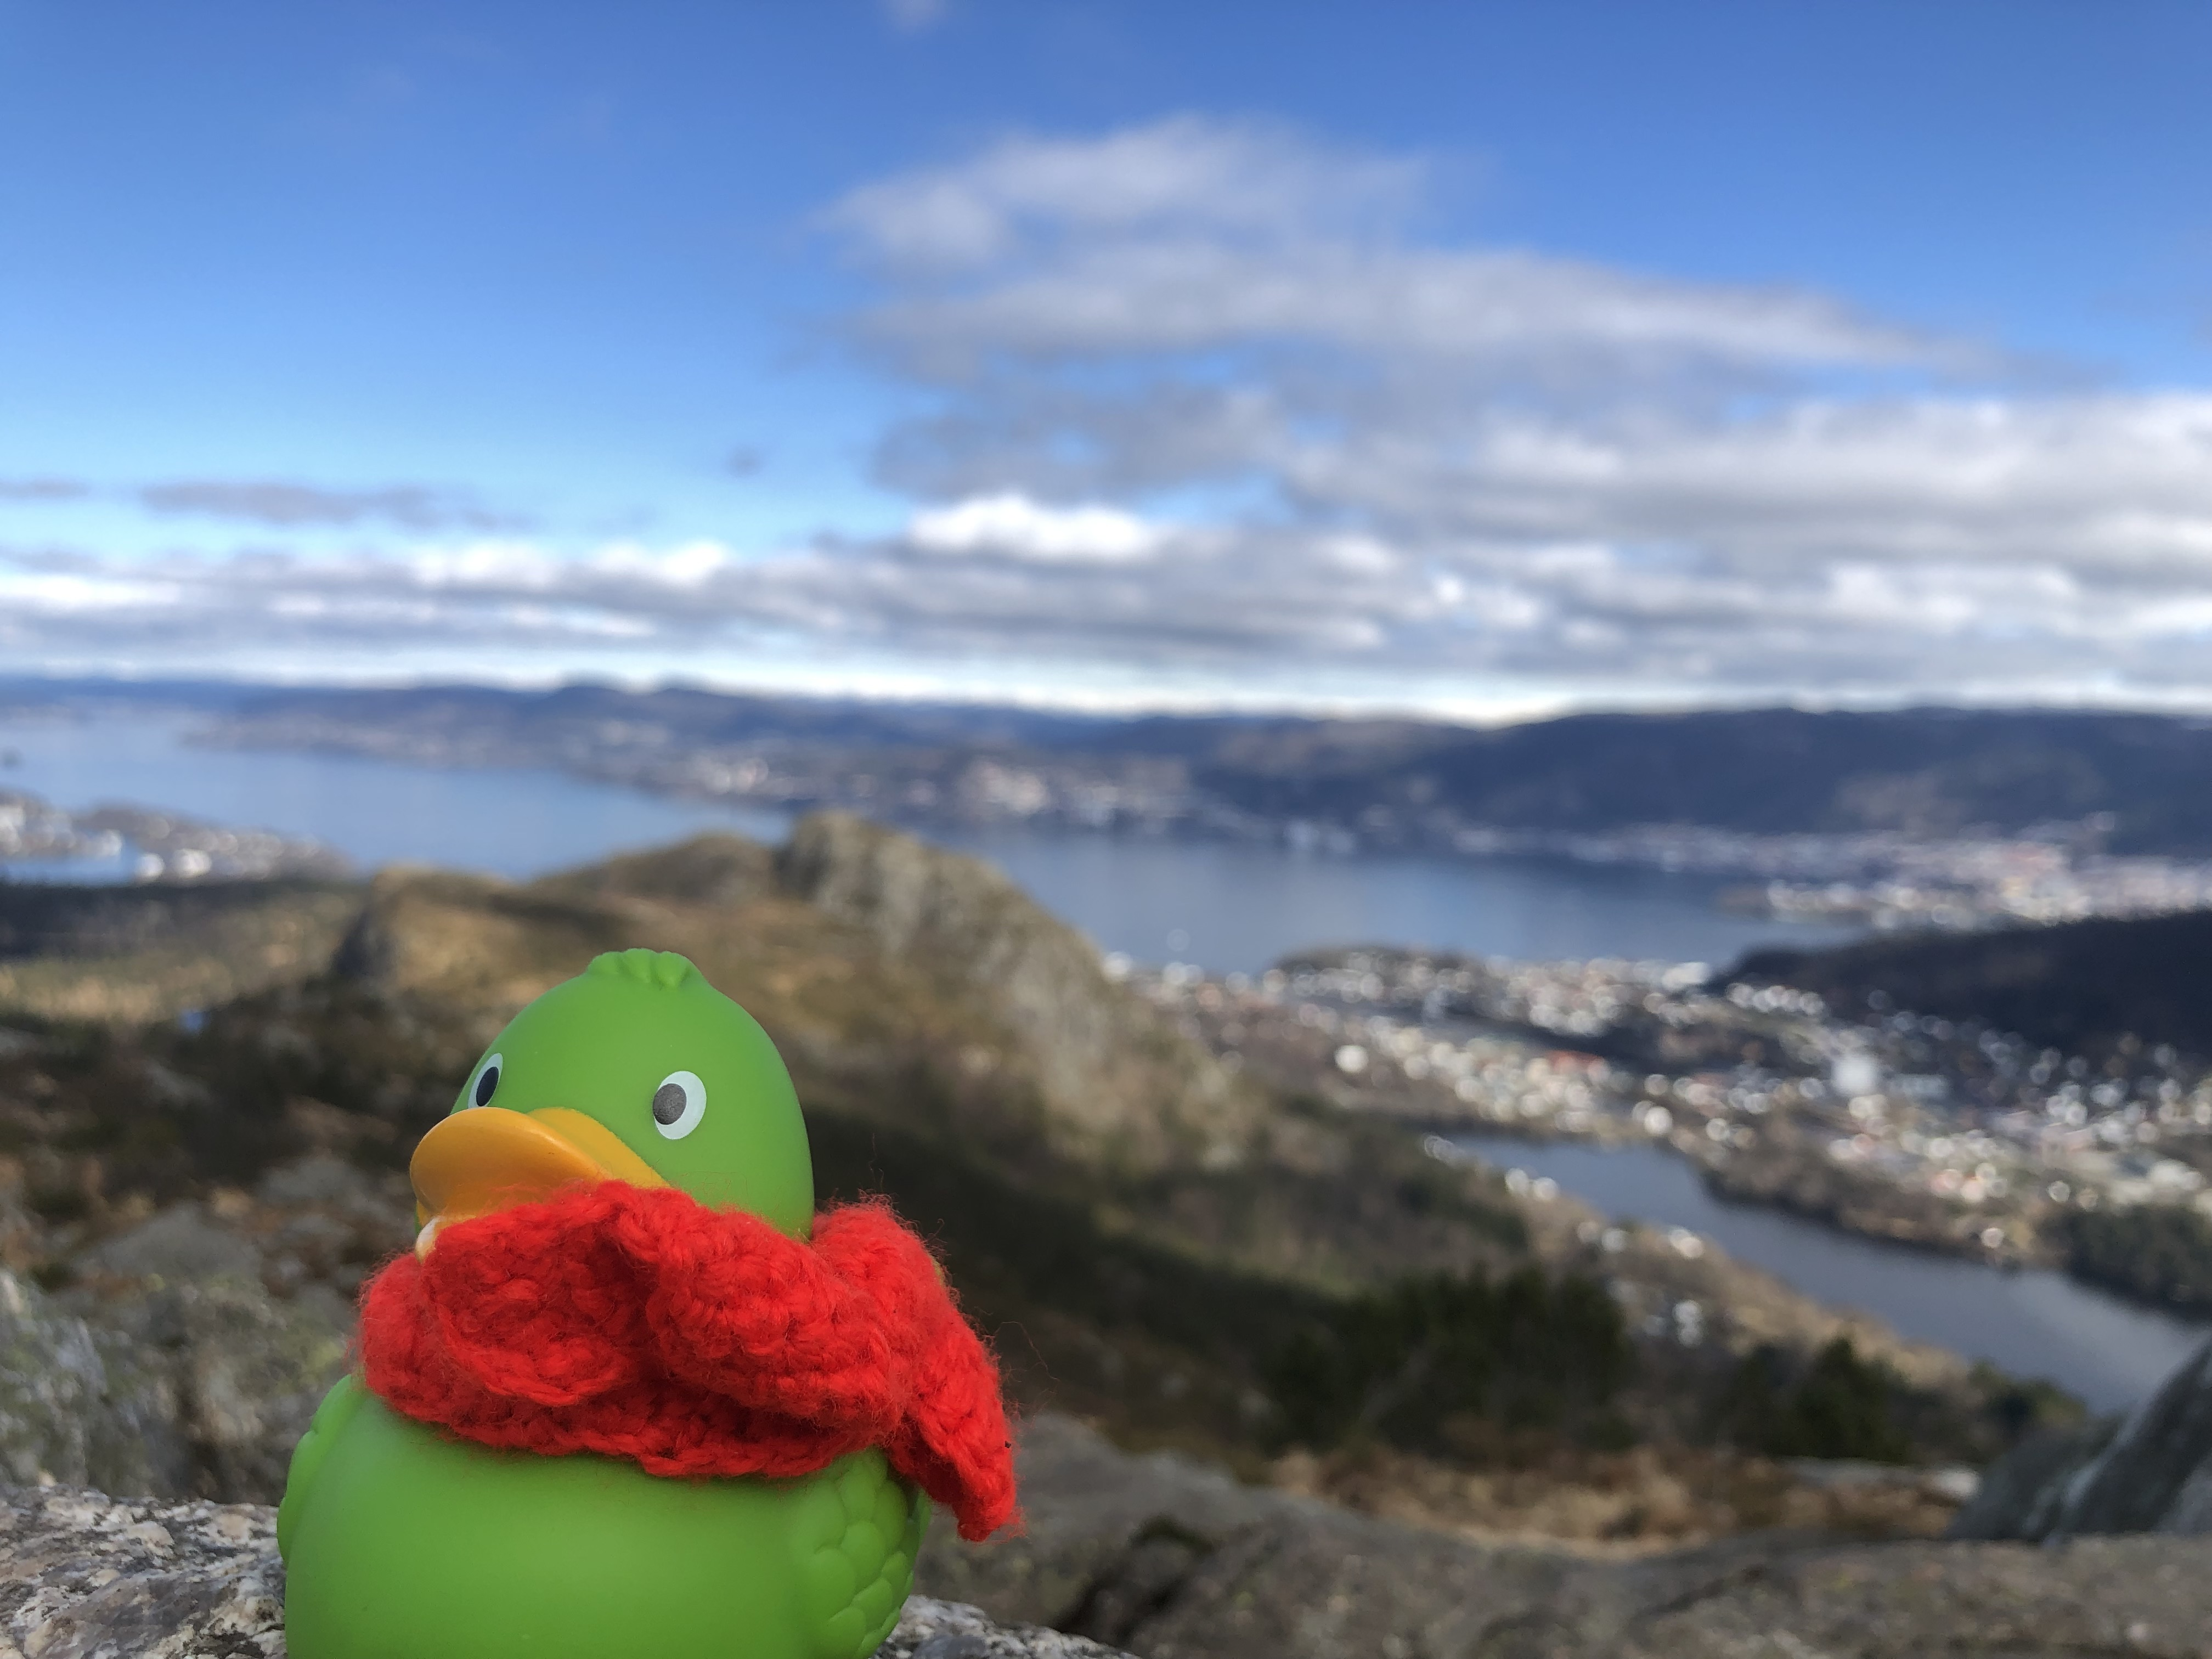
\includegraphics[height = 4.9cm]{images/guillaume8.jpg}
        \caption{Guillaume på Lyderhorn}
        \label{fig:guillaume8}
    \end{figure}
\end{frame}

%\section{Stokastisitet}
\subsection{Counting}
\begin{frame}
\begin{block}{Produktregelen}
\begin{itemize}
\item Noe kan brytes ned i to aksjoner som kombineres med hverandre
\item For den ene finnes det $n_1$ muligheter, for den andre $n_2$
\item Det blir $n_1\cdot n_2$ kombinasjoner
\end{itemize}
\end{block}
\pause
\begin{block}{Eksempel}
\begin{itemize}
\item Det er to type maskiner som trenges
\item Den ene finnes 3 ganger, den andre 5 ganger
\item Hvor mange kombinasjoner maskintype 1, maskintype 2 finnes det?
\item $5\cdot 3=15$
\end{itemize}
\end{block}
\end{frame}

\begin{frame}
\begin{block}{Sumregelen}
\begin{itemize}
\item Noe kan gjøres på enten en av $n_1$ måter, eller en av $n_2$ måter
\item Det finnes ingen element som er både i $n_1$ og i $n_2$
\item Det blir $n_1+n_2$ muligheter å gjøre det
\end{itemize}
\end{block}
\pause
\begin{block}{Eksempel}
\begin{itemize}
\item En student skal velge masteroppgaven sin
\item Hun liker tre fagområder
\item I område $n_1$ finnes det 5 temaer, i $n_2$ 3 temaer, i område $n_3$ er det 8
\item Det er $5+3+8=16$ temaer å velge fra
\end{itemize}
\end{block}
\end{frame}

\begin{frame}
\begin{block}{Substraksjonsregelen}
\begin{itemize}
\item Ligner \textit{Sumregelen}, men flere elementer er i flere grupper
\item Noe kan gjøres på enten en av $n_1$ måter, eller en av $n_2$ måter, men noen er i både $n_1$ og $n_2$
\item Det blir $n_1+n_2-felles(n_1,n_2)$ muligheter
\end{itemize}
\end{block}
\pause
\begin{block}{Eksempel}
\begin{itemize}
\item På fredag er det amerikansk-norsk folkefest
\item Det er 22 amerikanere og 18 nordmenn som meldte seg på
\item 3 av dem er både norsk og amerikansk
\item Det er $22+18-3=37$ personer som deltar
\end{itemize}
\end{block}
\end{frame}

\begin{frame}
\begin{block}{Divisjonsregelen}
\begin{itemize}
\item Det er $n$ måter å gjøre noe, men egentlig finnes det for hver måte minst $d$ lignende måter
\item Det blir da $n/d$ forskjellige muligheter
\end{itemize}
\end{block}
\pause
\begin{block}{Eksempel}
\begin{itemize}
\item I en fornøyelsespark for katter blir det talt 400 bein \item Mennesker og andre dyr har ikke lov å være i fornøyelsesparken
\item Hver katt har eksakt fire bein
\item Det betyr det er $400/4=100$ katter
\end{itemize}
\end{block}
\end{frame}

\begin{frame}[fragile]{Permutasjon? Kombinasjon? Variasjon? Hæ?}
\adjustbox{scale=0.9}{
\begin{tikzcd}
                               &                                                         & \text{Blir alle elementer med?} \arrow[ld, "ja"'] \arrow[rd, "nei"] &                                                                  &              \\
                               & \text{Permutasjon} \arrow[ld, "med"'] \arrow[d, "uten"] &                                                                    & \text{Er rekkefølgen viktig?} \arrow[ld, "ja"'] \arrow[d, "nei"] &              \\
 \frac{n!}{r!\cdot s!\cdot t!} & n!                                                      & \text{Variasjon} \arrow[ld, "med"'] \arrow[d, "uten"]              & \text{Kombinasjon} \arrow[d, "med"'] \arrow[rd, "uten"]          &              \\
                               & n^k                                                     & \frac{n!}{(n-k)!}                                                  & \binom{(n+k-1)}{(k-1)}                                           & \binom{n}{k}
\end{tikzcd}
}
\end{frame}


\begin{frame}{Eksempler}
\begin{block}{Eksempel 1}
\begin{itemize}
\item 6 personer må fotograferes. Hvor mange kombinasjoner finnes det å ordne dem på bildet?
\item Alle elementer blir med, ingen repetisjon 
\item Permutasjon uten repetisjon: $n!=6!=720$
\end{itemize}
\end{block}
\pause
\begin{block}{Eksempel 2}
\begin{itemize}
\item Hvor mange måter finnes det for å ordne bokstavene \textit{Mississippi}?
\item Alle elementer blir med, men repetisjon (permutasjon)
\item $\frac{n!}{r!\cdot s!\cdot t!} =  \frac{11!}{4!\cdot 4!\cdot 2!}=34650$
\end{itemize}
\end{block}
\end{frame}

\begin{frame}{Enda flere eksempler}
\begin{block}{Eksempel 3}
\begin{itemize}
\item Det er 7 personer og 3 tilfeldige av dem skal få en pris. Hvor mange kombinasjoner finnes det?
\item Ikke alle elementer blir med, ingen repetisjon, rekkefølgen ikke viktig 
\item Kombinasjon uten repetisjon: $\binom{n}{k}=\binom{7}{3}=\frac{7!}{3!\cdot 4!}=35$
\end{itemize}
\end{block}
\pause
\begin{block}{Eksempel 4}
\begin{itemize}
\item Vi har 5 typer is og skal spise 3 av dem. Vi er opptatt av rekkefølgen for best smak.
\item Ikke alle elementer blir med, rekkefølge viktig, med repetisjon
\item $n^k=5^3=125$
\end{itemize}
\end{block}
\end{frame}

\subsection*{Spørretid}
\begin{frame}{Spørsmål?}
    \begin{figure}
        \centering
        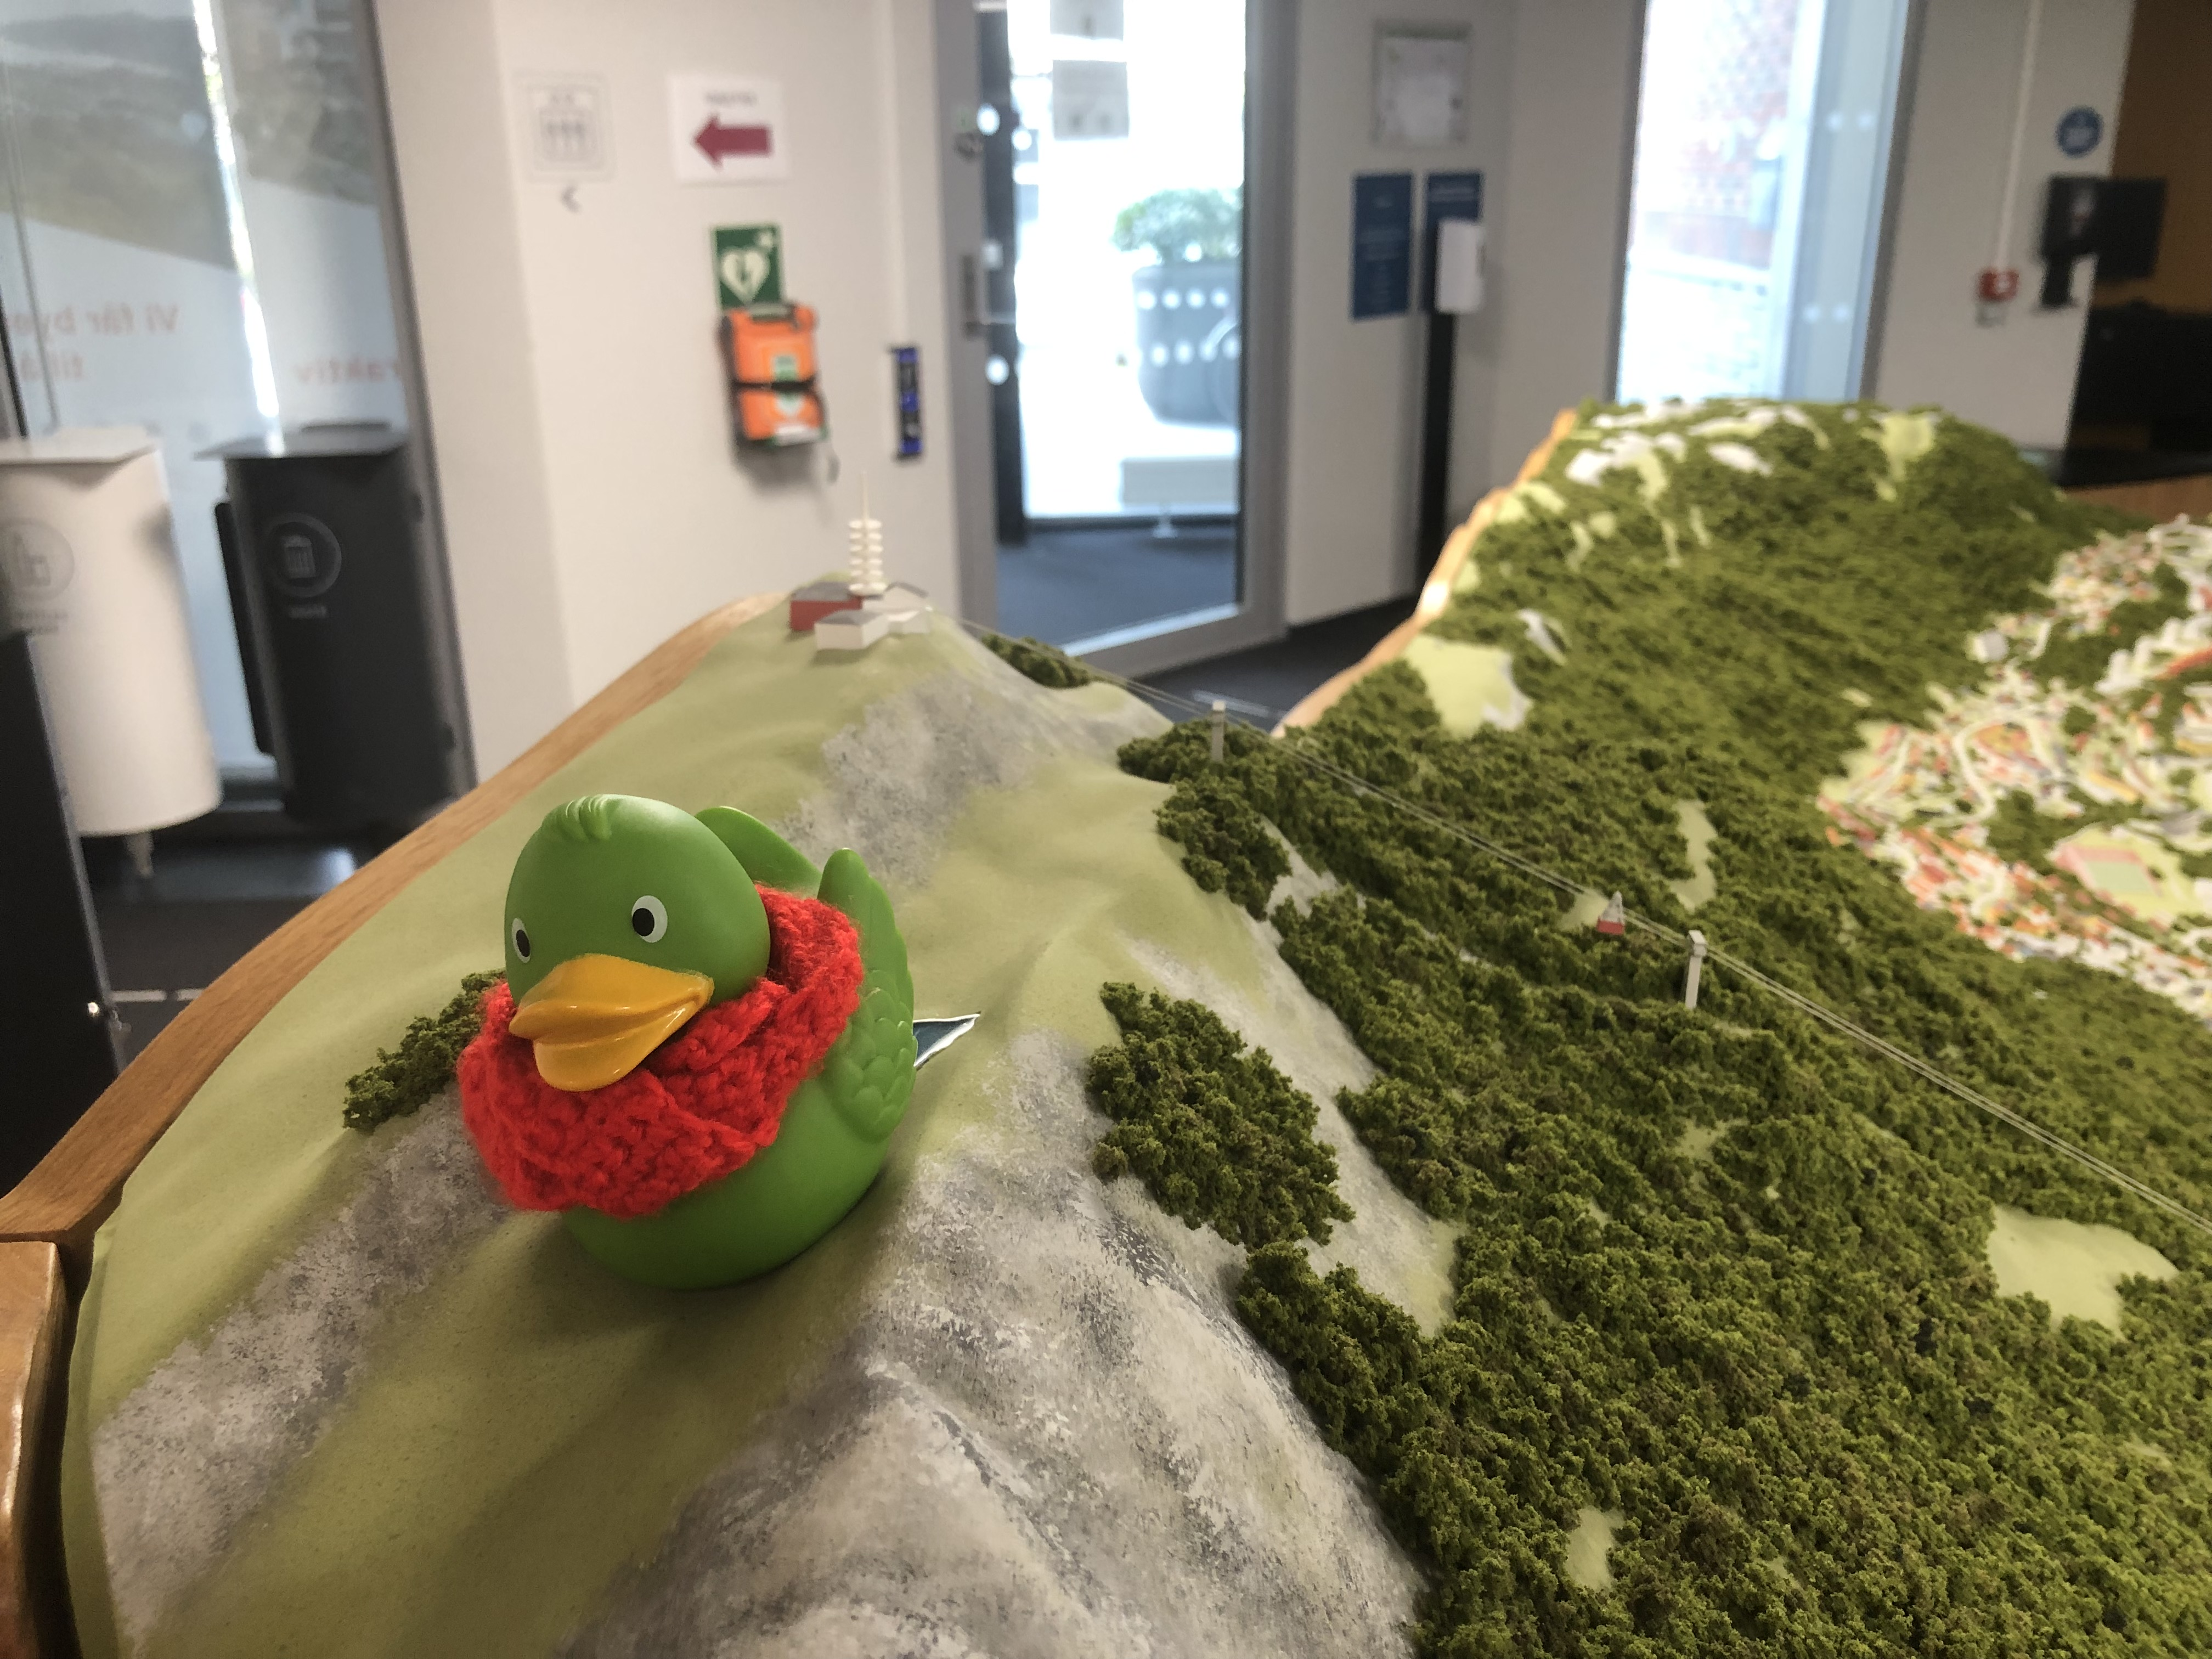
\includegraphics[height = 4.9cm]{images/guillaume11.jpg}
        \caption{Guillaume på Ulriken}
        \label{fig:guillaume11}
    \end{figure}
\end{frame}

\subsection{Sannsynligheter}
\begin{frame}{Definisjoner}
\begin{itemize}[<+->]
\item \textbf{Utfallsrom: }Alle mengder som har en sannsynlighet
\item \textbf{S: }Alle mulige utfall
\item \textbf{E: }Alle ønskete utfall
\item $E \subseteq S$: alle ønskete utfall er en del av alle mulige utfall
\item \textbf{Sannsynlighet: }$P(E)=\frac{|E|}{|S|}$
\item $0 \leq P(E) \leq 1$
\item $P(S)=1$
\item $P(\overline{E})=1-P(E)$
\end{itemize}
\end{frame}

\begin{frame}{Regneregler}
\begin{itemize}[<+->]
\item $P(A\cup B)=P(A)+P(B)-P(A\cap B)$ (tilsvarer subtraction rule)
\item $P(A\cap B)=P(A)\cdot P(B)$ hvis A,B statistisk uavhengig (tilsvarer multiplication rule)
\item $\sum_{s\in S} P(s) = 1 $ (summen av alle ting som kan skje har sannsynlighet 1)
\item \textbf{Betinget sannsynlighet: }$P(A|B)=\frac{P(A\cap B)}{P(B)}$ (Sannsynlighet av A etter at B skjedde)
\item \textbf{Bayes Rule: }$P(A|B)=\frac{P(B|A)\cdot P(A)}{P(B)}$
\end{itemize}
\end{frame}

\begin{frame}{Eksempler}
\begin{block}{Terninger}
\begin{itemize}[<+->]
\item Det er to terninger, den ene er vanlig med 6 jevne sider
\item Den andre har tallene $\{3,4,5,5,6,6\}$
\item Hvor stor er sannsynligheten at vi kaster en 7 med begge terninger?
\item Det er $6\cdot 6$ mulige kombinasjoner
\item Det er fire måter å få det til:
\begin{itemize}
\item Terning 1: 1, Terning 2: 6 (finnes to ganger)
\item Terning 1: 2, Terning 2: 5 (finnes to ganger)
\item Terning 1: 3, Terning 2: 4
\item Terning 1: 4, Terning 2: 3
\end{itemize}
\item $P(sum=7)=\frac{6}{36}=\frac{1}{6}$
\end{itemize}
\end{block}
\end{frame}

\begin{frame}{Eksempler}
\begin{block}{Kortspill}
\begin{itemize}[<+->]
\item Vi har et vanlig tysk kortspill med 32 kort (4 farger, $\{7,8,9,10,J,Q,K,A\}$)
\item Hva er sannsynligheten at vi trekker et hjerte eller en konge?
\item Hva er sannsynligheten at en av disse kortene er 7,8 eller 9?
\item Det er 4 konger, 8 hjerter, en av dem er begge deler
\item $P(Konge\cup Hjerte)=\frac{8+4-1}{32}=\frac{11}{32}$
\item Blant disse er det 3 kort som er 7,8 eller 9
\item $P(7,8,9|Konge\cup Hjerte)=\frac{P((7,8,9)\cap(Konge\cup Hjerte))}{P(Konge\cup Hjerte)}=\frac{3}{32}\cdot \frac{32}{11}=\frac{3}{11}$
\end{itemize}
\end{block}
\end{frame}

\begin{frame}{\textit{Vierfeldertafel} (WANTED: norsk eller engelsk begrep)}
\begin{table}[h!]
\centering
\label{tab:prob_two_events}
\begin{tabular}{l|ll|l}
\cline{2-3}
                            & $A$            & $\overline{A}$            &                               \\ \hline
\multicolumn{1}{|l|}{$B$}   & $P(A\cap B)$   & $P(\overline{A}\cap B)$   & \multicolumn{1}{l|}{$P(B)$}   \\
\multicolumn{1}{|l|}{$\overline{B}$} & $P(A\cap \overline{B})$ & $P(\overline{A}\cap \overline{B})$ & \multicolumn{1}{l|}{$P(\overline{B})$} \\ \hline
                            & $P(A)$         & $P(\overline{A})$         & \multicolumn{1}{l|}{$1$}      \\ \cline{2-4} 
\end{tabular}
\caption{To hendelser A og B i en \textit{Vierfeldertafel}}
\end{table}
\pause
\begin{itemize}[<+->]
\item Det er to spalter og to rekker, hver for en hendelse og motsetningen
\item I alle retninger kan man summe ting sammen
\item Det trenges bare tre utfylte felter for å regne ut resten
\end{itemize}
\end{frame}

\begin{frame}{\textit{Vierfeldertafel} (WANTED: norsk eller engelsk begrep)}
\begin{columns}
 \begin{column}{0.38\textwidth}
\begin{table}[h!]
\centering
\caption{Eksempel \textit{Vierfeldertafel}}
\label{tab:fourfold_eksempel1}
\begin{tabular}{l|ll|l}
\cline{2-3}
                            & $A$            & $A^C$            &                               \\ \hline
\multicolumn{1}{|l|}{$B$}   & 0.4   &     & \multicolumn{1}{l|}{0.533}   \\
\multicolumn{1}{|l|}{$B^C$} &   & 0.292 & \multicolumn{1}{l|}{} \\ \hline
                            &          &          & \multicolumn{1}{l|}{$1$}      \\ \cline{2-4} 
\end{tabular}
\end{table}

\begin{table}[h!]
\centering
%\caption{Eksempel \textit{Vierfeldertafel} ferdig utfylt}
\label{tab:fourfold_eksempel2}
\begin{tabular}{l|ll|l}
\cline{2-3}
                            & $A$            & $A^C$            &                               \\ \hline
\multicolumn{1}{|l|}{$B$}   & 0.4   & 0.133    & \multicolumn{1}{l|}{0.533}   \\
\multicolumn{1}{|l|}{$B^C$} & 0.175  & 0.292 & \multicolumn{1}{l|}{0.467} \\ \hline
                            & 0.575         & 0.425         & \multicolumn{1}{l|}{$1$}      \\ \cline{2-4} 
\end{tabular}
\end{table}
 \end{column}
 \pause
 \begin{column}{0.58\textwidth}
\begin{itemize}[<+->]
\item Det er gitt tre verdier, $P(B)$, $P(A\cap B)$, $P(A^C\cap B^C)$
\item Resten kan regnes ut ved summeformalen
\item Eksempel: $P(A^C\cap B)=P(A\cap B)-P(B)=0.533-0.4=0.133$
\item Kan brukes for å finne andre ting
\item Betinget sannsynlighet: $P(A|B)=\frac{P(A\cap B)}{P(B)}=\frac{0.4}{0.533}=0.75$
\end{itemize}
 \end{column}
\end{columns}
\end{frame}

\begin{frame}[fragile]{Sannsynlighetstre}
\begin{tikzcd}
           &                                                         & {} \arrow[ld, "P(A)" description] \arrow[rd, "P(\overline{A})" description] &                                                                               &                                   \\
           & {} \arrow[ld, "P(B|A)"'] \arrow[d, "P(\overline{B}|A)"] &                                                                             & {} \arrow[d, "P(B|\overline{A})"'] \arrow[rd, "P(\overline{B}|\overline{A})"] &                                   \\
P(A\cap B) & P(A \cap \overline{B})                                  &                                                                             & P(\overline{A} \cap B)                                                        & P(\overline{A} \cap \overline{B})
\end{tikzcd}
\end{frame}

\begin{frame}[fragile]{Sannsynlighetstre}
\begin{tikzcd}
    &                                                         & {} \arrow[ld, "0.575" description] \arrow[rd, "0.425" description] &                                                                               &       \\
    & {} \arrow[ld, "P(B|A)"'] \arrow[d, "P(\overline{B}|A)"] &                                                                    & {} \arrow[d, "P(B|\overline{A})"'] \arrow[rd, "P(\overline{B}|\overline{A})"] &       \\
0.4 & 0.175                                                   &                                                                    & 0.133                                                                         & 0.292
\end{tikzcd}
\end{frame}

\begin{frame}[fragile]{Sannsylighetstre}
\begin{tikzcd}
    &                                            & {} \arrow[ld, "0.575" description] \arrow[rd, "0.425" description] &                                            &       \\
    & {} \arrow[ld, "0.696"'] \arrow[d, "0.304"] &                                                                    & {} \arrow[d, "0.313"'] \arrow[rd, "0.687"] &       \\
0.4 & 0.175                                      &                                                                    & 0.133                                      & 0.292
\end{tikzcd}
\end{frame}
\subsection*{Spørretid}
\begin{frame}{Spørsmål?}
    \begin{figure}
        \centering
        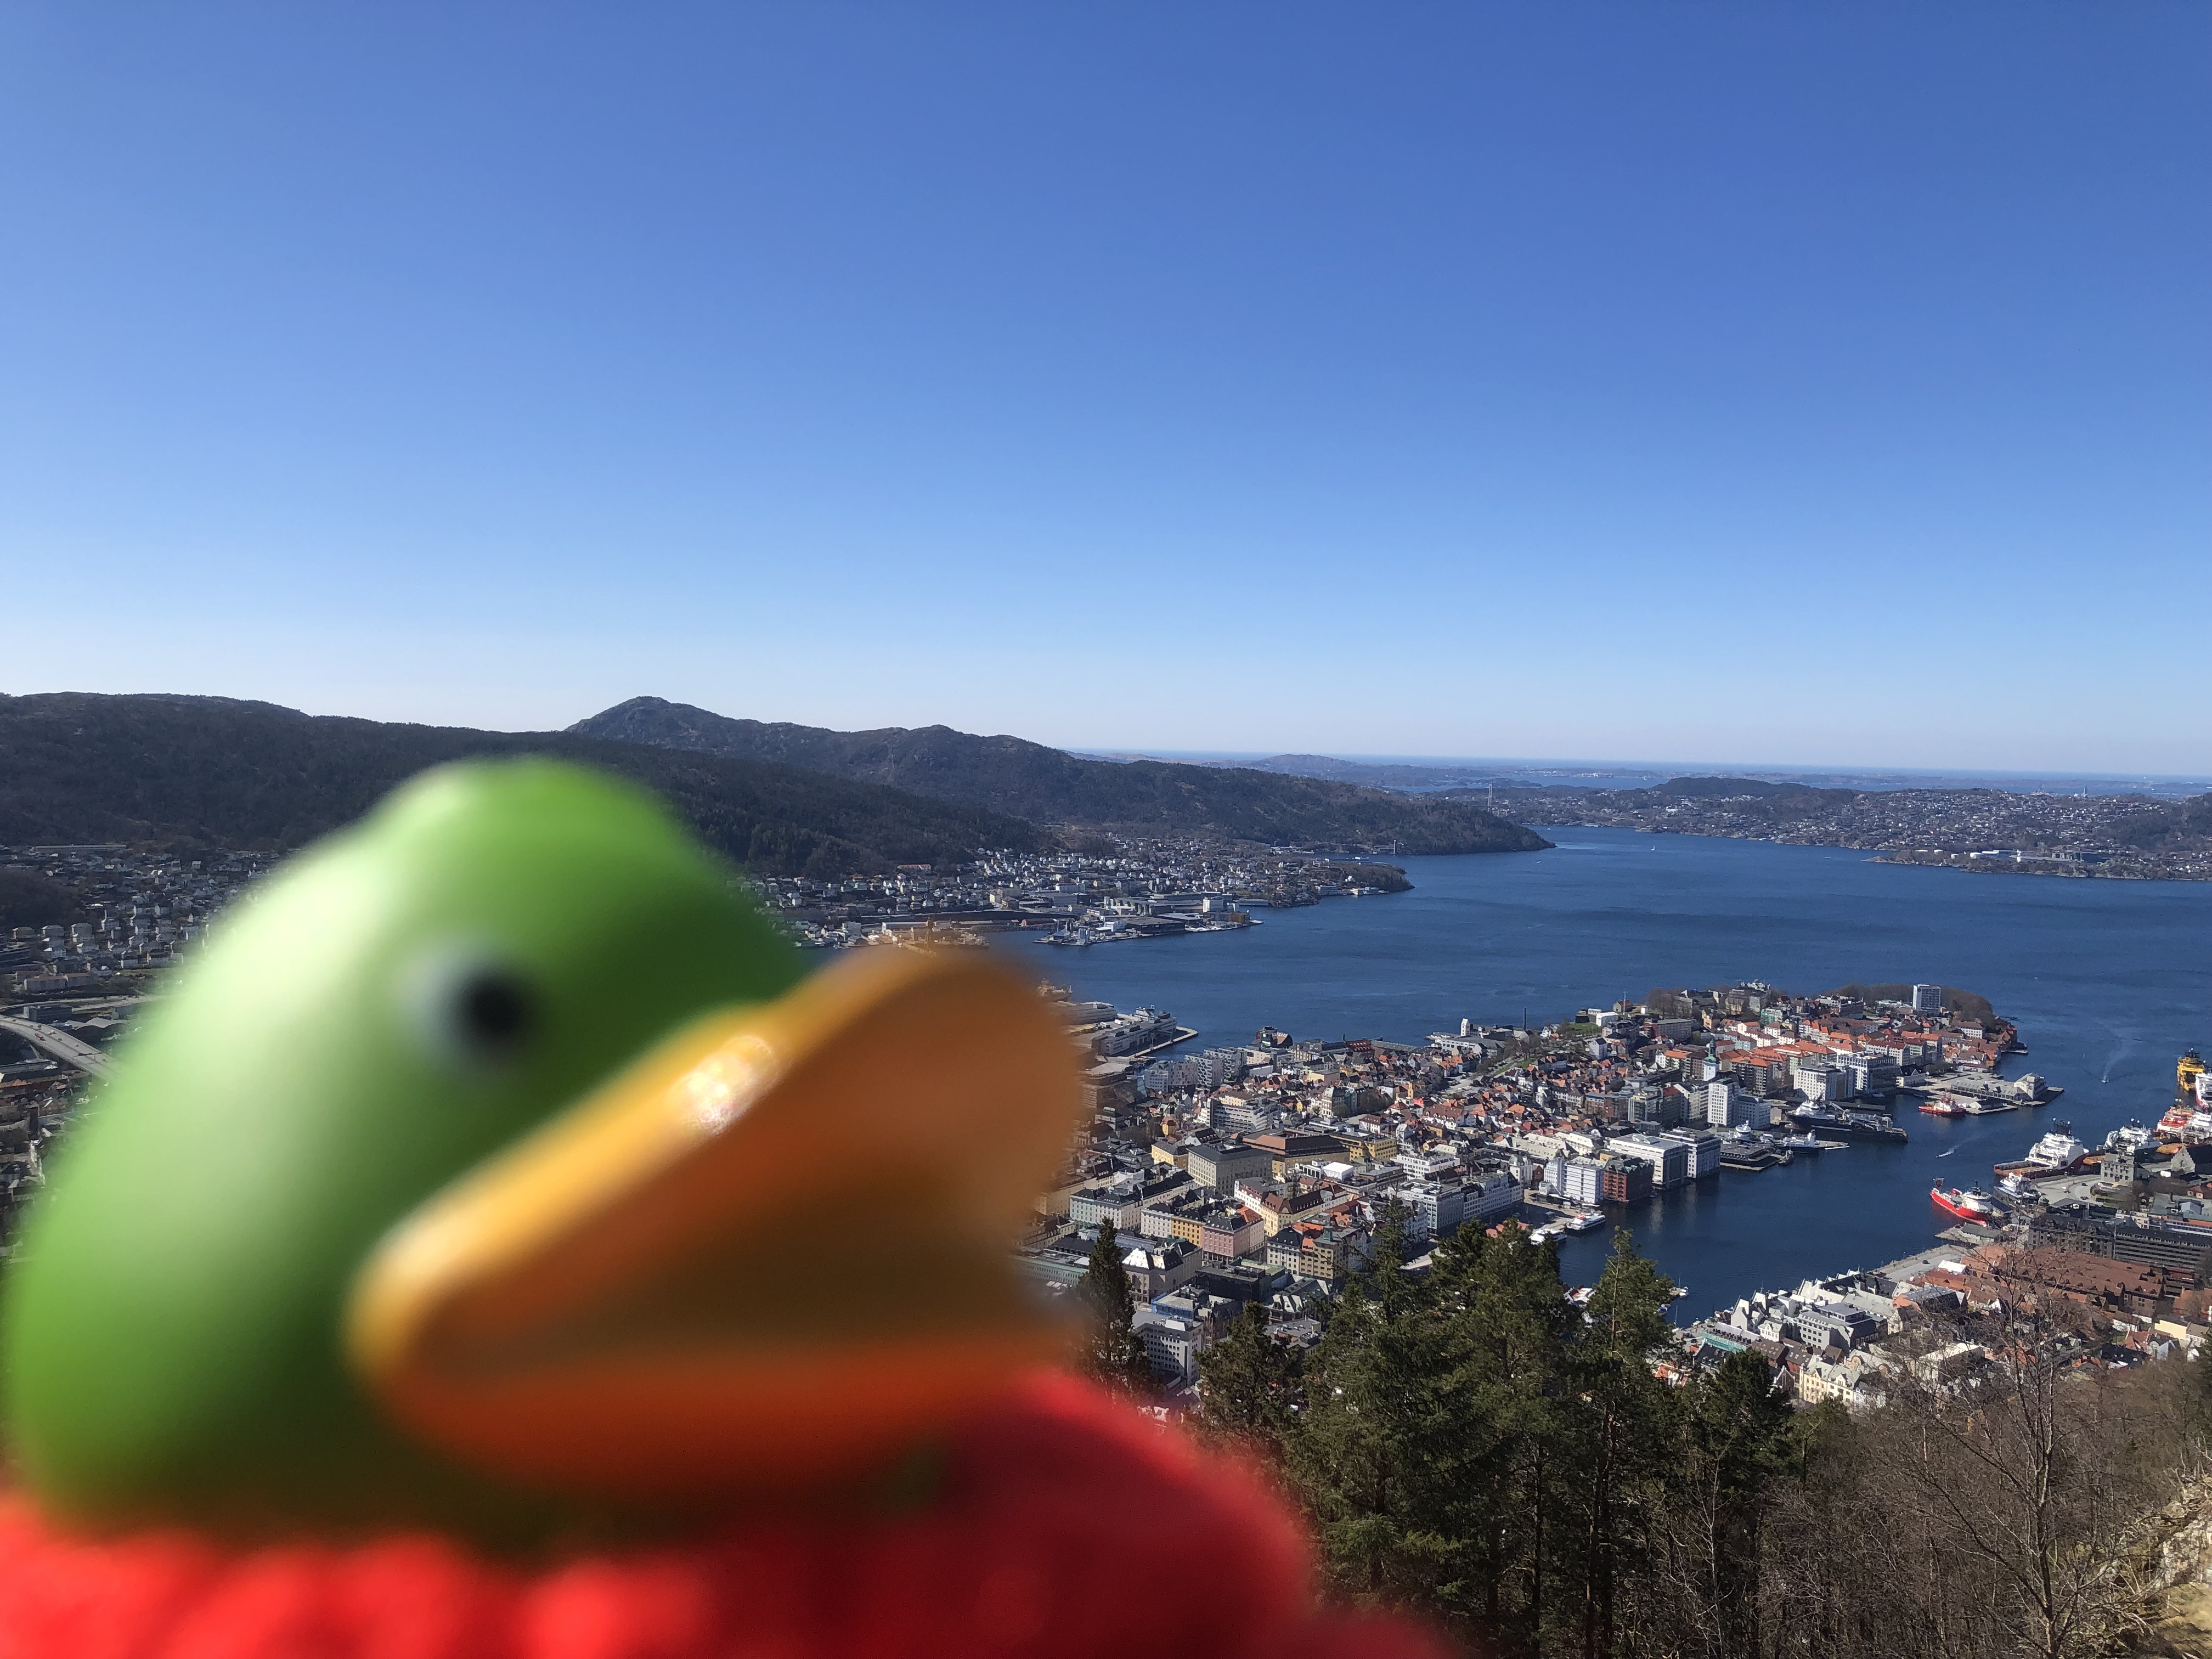
\includegraphics[height = 4.9cm]{images/guillaume10.jpg}
        \caption{Guillaume på Fløyen}
        \label{fig:guillaume10}
    \end{figure}
\end{frame}



\section{Algoritmer}

\subsection{Kompleksitet}
\begin{frame}[fragile]{Kompleksitet}
    Gitt to algoritmer som løser det samme problemet, hvordan vite hvilken som er kjappest?
    %Vi kan kjøre begge to og ta tiden, men det hadde vært kjekt å vite svaret før vi bruker tid på å implementere noe som helst.
    \begin{columns}
        \begin{column}{0.45\textwidth}
            \begin{minted}[fontsize=\scriptsize]{python}
def minAndMax(list):
    min = list[0]
    for elem in list[1:]:
        if elem < min:
            min = elem
    max = list[0]
    for elem in list[1:]:
        if elem > max:
            max = elem
    return (min, max)
            \end{minted}
        \end{column}
        \pause
        \begin{column}{0.45\textwidth}
            \begin{minted}[fontsize=\scriptsize]{python}
def minAndMax(list):
    min, max = list[0], list[0]
    for elem in list[1:]:
        if elem < min: min = elem
        if elem > max: max = elem
    return (min, max)
    
def minAndMax(list):
    list = sorted(list)
    return (list[0], list[-1])
            \end{minted}
        \end{column}
    \end{columns}    
\end{frame}
\begin{frame}[fragile]{}
    Hvis vi hadde testet alle tre algoritmene på mange lister av økende lengde, ville det kanskje sett slik ut. Hvorfor?
    \begin{figure}
        \centering
        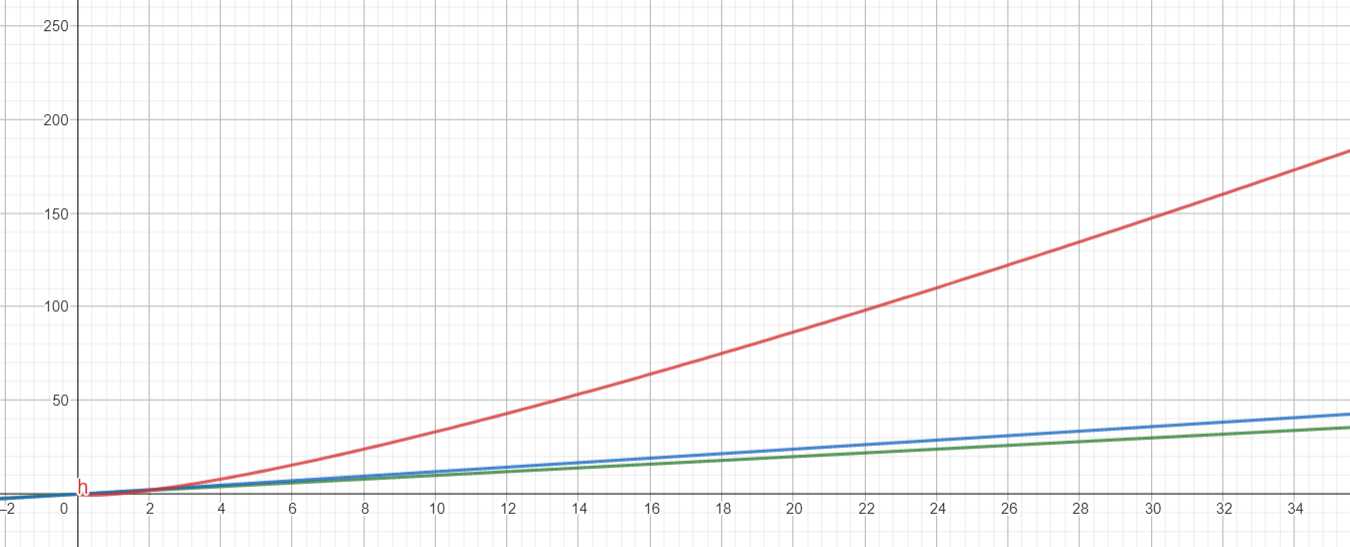
\includegraphics[height = 4.5cm]{images/minmax.png}
        \caption{Den røde er den som sorterer.}
        \label{fig:minmax}
    \end{figure}    
\end{frame}

\begin{frame}[fragile]{}
    La oss si at listen har en lengde på $n$. Hvor mange operasjoner blir det?
    \begin{columns}
        \begin{column}{0.45\textwidth}
            \begin{minted}[fontsize=\scriptsize]{python}
def minAndMax(list):
    min = list[0]         # 1
    for elem in list[1:]: # n-1
        if elem < min:    # 1
            min = elem    # 1
    max = list[0]         # 1
    for elem in list[1:]: # n-1
        if elem > max:    # 1
            max = elem    # 1
    return (min, max)
            \end{minted}
            Det blir ca $1 + (n-1)*(1+1) + 1 + (n-1)*(1+1) = 2 + 4*(n-1) = 4n-2$, og det er ihvertfall mindre enn \underline{$100n$}.
        \end{column}
        \pause
        \begin{column}{0.45\textwidth}
            \begin{minted}[fontsize=\scriptsize]{python}
def minAndMax(list):              
    min, max = list[0], list[0]   # 2
    for elem in list[1:]:         # n-1
        if elem < min: min = elem # 2
        if elem > max: max = elem # 2
    return (min, max)
    
def minAndMax(list):
    list = sorted(list)    # n * log2(n)
    return (list[0], list[-1]) # 2
            \end{minted}
            Den første blir $2+(n-1)*(2+2) = 2+4(n-1) = 4n-2$, som er mindre enn \underline{$100n$}.\\
            \pause
            Den andre blir $2 + n \cdot log_2(n)$, og det er mindre enn \underline{$100 \cdot n \cdot log_2(n)$}.
        \end{column}
    \end{columns}
\end{frame}

\begin{frame}{Big O}
    Nå skal vi formalisere konseptet om hvor godt noe skalerer.
    \begin{definition}[Big O]
        Gitt to funksjoner $f, g : \mathbb{N} \rightarrow \mathbb{N}$: \\
        Hvis $\exists c, n_0 : \forall n > n_0 : [ f(n) \leq c*g(n) ]$, da er $f = O(g)$.\\
        Intuitivt kan vi tenke at $f \leq g$.
    \end{definition}
    \pause
    I vårt eksempel fant vi at algoritmene bruker mindre enn $100n$, $100n$, og $100 \cdot n \cdot log_2(n)$ operasjoner, og da kjører algoritmene på $O(n)$, $O(n)$, og $O(n \cdot log(n))$.\\[2mm]
    Big O er en veldig kjapp og enkel måte å estimere hva slags forskjeller som betyr noe og ikke. Konstanter spiller nesten ingen rolle i det store bildet: $O(10n) = O(5n) = O(n)$.
\end{frame}

\begin{frame}[fragile]{Regneregler for Big O}
    Løkker gjør at innholdet blir gjort mange ganger, da ganger vi med innholdet.
    \begin{minted}[fontsize=\scriptsize]{python}
for _ in range(n):     # O(n)
    for _ in range(m): # O(m)
        do_something() # O(1)
# Total: O(n)*O(m)*O(1) = O(nm).
    \end{minted}
    \pause
    Om vi vil summere flere ting, tar vi det største. Om vi ikke vet hva som er størst beholder vi begge.  
    \begin{columns}
        \begin{column}{0.45\textwidth}
            \begin{minted}[fontsize=\scriptsize]{python}
    for _ in range(n): # O(n)
        do_something() # O(1)
    do_something()     # O(1)
    do_something()     # O(1)
    # Total: O(n) + O(1) + O(1) = O(n).  
            \end{minted}
        \end{column}
        \pause
        \begin{column}{0.45\textwidth}
            \begin{minted}[fontsize=\scriptsize]{python}
    for _ in range(n): # O(n)
        do_something() # O(1)
    for _ in range(m): # O(m)
        do_something() # O(1)
    # Total: O(n) + O(m) = O(n+m).
            \end{minted}
            
        \end{column}
    \end{columns}
\end{frame}

\subsection{Søking}
\begin{frame}[fragile]{Søking}
    Big O er pessimistisk, og bryr seg kun om det verste tenkelige tilfellet.
    \begin{minted}[fontsize=\scriptsize]{python}
def index_of(list, e):
    for i in range(len(list)): # O(n)
        if list[i] == e:       # O(1)
            return i           # O(1)
    return -1                  # Total: O(n)
    \end{minted}
    Summen er fortsatt $O(n)$, selv om det er mulig vi blir ferdig tidligere.
\end{frame}

\begin{frame}[fragile]{Binærsøk}
    \begin{columns}
        \begin{column}{0.50\textwidth}
            \begin{figure}
                \centering
                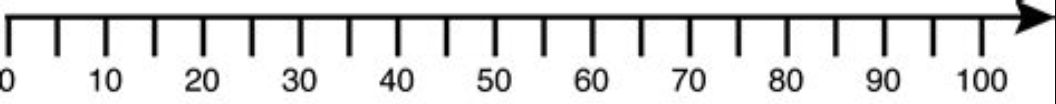
\includegraphics[scale=0.3]{images/Tallinje.png}
                \label{fig:tall}
            \end{figure}  
            \pause
            \begin{minted}[fontsize=\scriptsize]{python}
def binary_search(list, target):
    left = 0
    right = len(arr) - 1
    while left <= right:
        mid = (left + right) // 2
        if arr[mid] == target: return mid
        elif arr[mid] < target: left = mid + 1
        else: right = mid - 1
    return -1
            \end{minted}       
        \end{column}
        \begin{column}{0.47\textwidth}
            Hvor mange operasjoner blir det?\\\pause
            Vi må finne ut hvor mange ganger løkken looper.\\\pause
            I hver iterasjon blir avstanden mellom $left$ og $right$ halvert, og det kan gjøres $log_2(n)$ ganger før vi kommer til 0 eller 1.\\[2mm]\pause
            Dermed kjører binærsøk i $log_2(n)$, som er veldig mye bedre enn $O(n)$.
        \end{column}
    \end{columns}
\end{frame}
%\section{Grafer}

\begin{frame}[fragile]{Grafer}
    Veldig mange algoritmeproblemer kan representeres som grafer.
    \begin{columns}
        \begin{column}{0.3\textwidth}
            \begin{figure}
                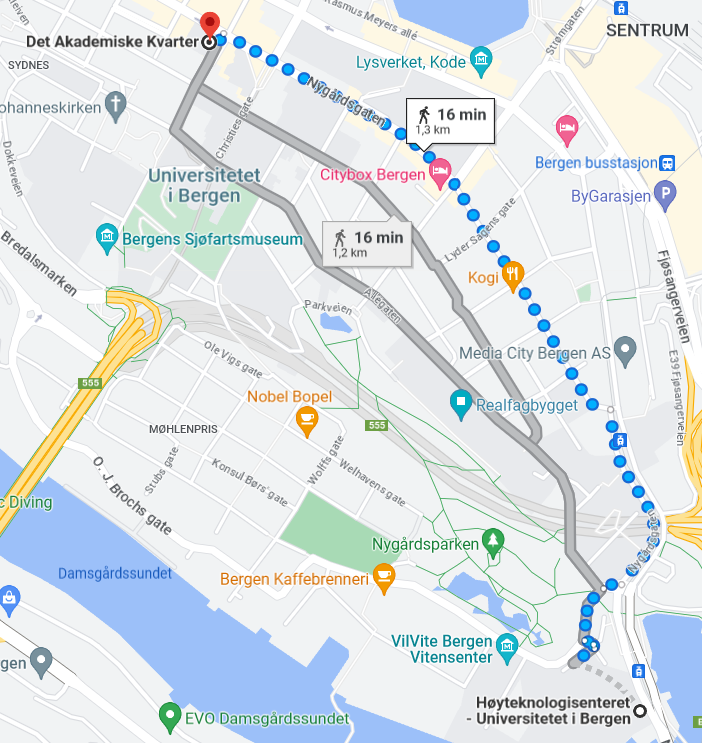
\includegraphics[width=4cm]{images/Kvarteret.png}
                \caption{Hva er kjappeste veien til Kvarteret?}
            \end{figure}
        \end{column}
        \begin{column}{0.3\textwidth}
            \begin{figure}
                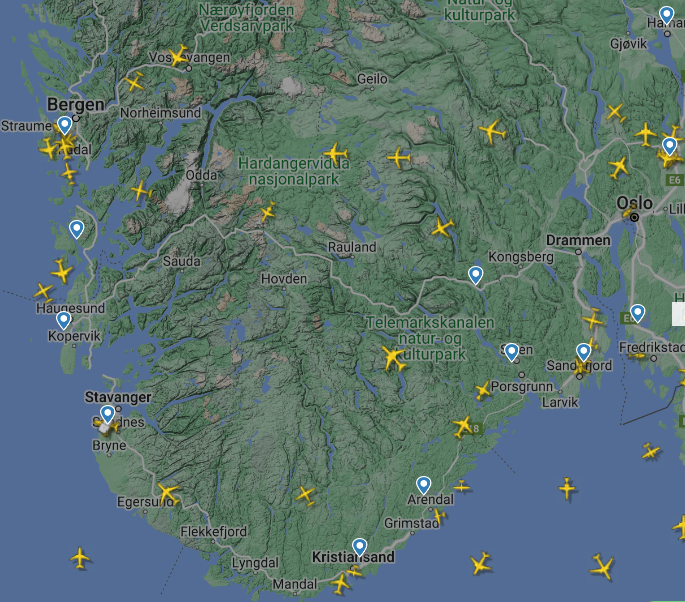
\includegraphics[width=4cm]{images/Bergen.png}
                \caption{Hvilke fly kan du ta for å komme deg hjem fortest?}
            \end{figure}
        \end{column}
        \begin{column}{0.3\textwidth}
            \begin{tikzcd}
                                  & b \arrow[rr, no head] &                                           & e \arrow[loop, distance=2em, in=305, out=235] \\
            a \arrow[rr, no head] &                       & d \arrow[lu, no head] \arrow[ld, no head] &                                               \\
                                  & c \arrow[lu, no head] &                                           &                                              
            \end{tikzcd}
        \end{column}
    \end{columns}
\end{frame}


\subsection*{Begreper}
\begin{frame}
    \begin{block}{Graf $G(V,E)$}
    En Graf $G = (V, E)$ er et par av et sett noder (vertices) $V$ og et sett av kanter (edges) $E$.
    \end{block}
    \pause

\begin{columns}
    \begin{column}{0.28\textwidth}
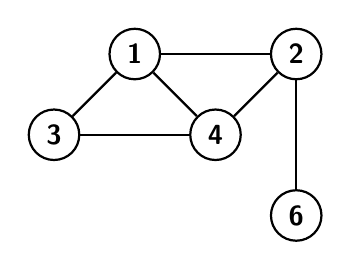
\begin{tikzpicture}[
    node distance=1.45cm, thick,
    main node/.style={circle, draw, font=\sffamily\bfseries}
]
    \node[main node] (1)                    {1};
    \node[main node] (3) [below left  of=1] {3};
    \node[main node] (4) [below right of=1] {4};
    \node[main node] (2) [above right of=4] {2};
    \node[main node] (6) [below right of=4] {6}; % <-4> forces an additional overlay in which node 2 disappears

    \path (1) edge (2)
        (4) edge (2)
        (6) edge (2);
    \path (1) edge (3)
        (4) edge (1);
    \path (3) edge (4);
\end{tikzpicture}
 \end{column}
 \pause
    \begin{column}{0.68\textwidth}
\begin{itemize}[<+->]
    \item Noder: $V=\{1,2,3,4,6\}$ \pause
    \item Kanter: $E=\{(1,2), (1,4), (3,4), (2,4), (2,6), (1,3)\}$\pause
    \item Sti (/path): Vei fra A til B\\
    Eksempel: $Path(1,6)=[1,2,6]$\pause
    \item Sykel (/Cycle): En sti med samme start og slutt\\
    Eksempel: $[1,3,4,1]$, $[1,2,4,3,1]$\pause
    \item Nabolag: Alle naboene en node kan nå med én kant\\
    Eksempel: $N(4)={1,2,3}$, $N(6)=2$\pause
    \item Grad (/degree): Antall naboer av en node\\
    Eksempel: $deg(4)=3$, $deg(6)=1$
\end{itemize}
 \end{column}
\end{columns}
\end{frame}

\begin{frame}{Rettede grafer}
    Om du skal lage en graf av veinettverket i Bergen, får du fort problemer. Hele sentrum er jo enveiskjørt! Vi trenger å kunne representere enveiskanter.
    \begin{columns}
    \begin{column}{0.48\textwidth}
    \begin{figure}
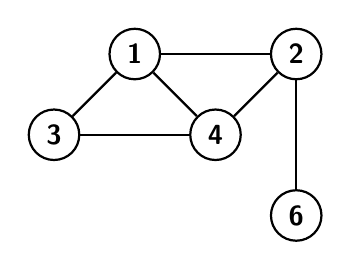
\begin{tikzpicture}[
    node distance=1.45cm, thick,
    main node/.style={circle, draw, font=\sffamily\bfseries}
]
    \node[main node] (1)                    {1};
    \node[main node] (3) [below left  of=1] {3};
    \node[main node] (4) [below right of=1] {4};
    \node[main node] (2) [above right of=4] {2};
    \node[main node] (6) [below right of=4] {6}; % <-4> forces an additional overlay in which node 2 disappears

    \path (1) edge (2)
        (4) edge (2)
        (6) edge (2);
    \path (1) edge (3)
        (4) edge (1);
    \path (3) edge (4);
\end{tikzpicture}
\caption{Urettet graf (undirected).\\$deg(4) = 3$}
\end{figure}
 \end{column}
 \pause
    \begin{column}{0.48\textwidth}
    \begin{figure}
    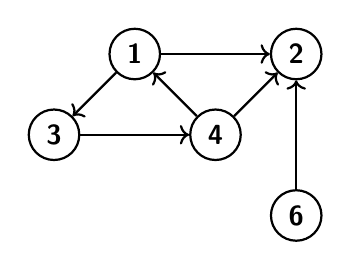
\begin{tikzpicture}[
    node distance=1.45cm, thick,
    main node/.style={circle, draw, font=\sffamily\bfseries}
]
    \node[main node] (1)                    {1};
    \node[main node] (3) [below left  of=1] {3};
    \node[main node] (4) [below right of=1] {4};
    \node[main node] (2) [above right of=4] {2};
    \node[main node] (6) [below right of=4] {6}; % <-4> forces an additional overlay in which node 2 disappears

    \path[->] (1) edge (2)
        (4) edge (2)
        (6) edge (2);
    \path[->] (1) edge (3)
        (4) edge (1);
    \path[->] (3) edge (4);
\end{tikzpicture}
\caption{Rettet graf (directed).\\ $deg^+(4) = 2$\\$deg^-(4) = 2$}
\end{figure}
 \end{column}
\end{columns}
\end{frame}

\begin{frame}
    \begin{block}{Bipartitte grafer $G(V,A,B)$}
    En bipartitt graf er en graf som kan deles i to sett $A,B$ der alle kanter $v\in V$ går fra en node i $A$ til en node i $B$. Grafen kan fargelegges i to farger slik at alle kanter går fra én farge til en annen farge.
    \end{block}

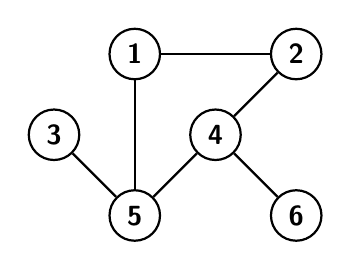
\begin{tikzpicture}[
    node distance=1.45cm, thick,
    main node/.style={circle, draw, font=\sffamily\bfseries}
]
    \node[main node,onslide=<2->{fill=black!40!green}] (1)                    {1};
    \node[main node,onslide=<2->{fill=black!40!green}] (3) [below left  of=1] {3};
    \node[main node,onslide=<2->{fill=black!40!green}] (4) [below right of=1] {4};
    \node[main node,onslide=<2->{fill=black!30!red}] (2) [above right of=4] {2};
    \node[main node,onslide=<2->{fill=black!30!red}] (5) [below right of=3] {5};
    \node[main node,onslide=<2->{fill=black!30!red}] (6) [below right of=4] {6};

    \path (1) edge (2)
        (1) edge (5)
        (3) edge (5)
        (4) edge (2)
        (4) edge (5)
        (4) edge (6);
\end{tikzpicture}
\end{frame}

\begin{frame}{Trær}
    \begin{itemize}
        \item Et \emph{tre} er en \textit{sammenhengende}, \textit{urettet} graf uten sykler.
        \item En \emph{skog} er en graf med flere trær som ikke er tilknyttet hverandre.
        \item Et \emph{blad} i et tre er en node som har grad 1.
        \item En \emph{intern node} i et tre er en node som ikke er et blad.
    \end{itemize}
    \pause
    \begin{columns}
    \begin{column}{0.48\textwidth}
\begin{figure}
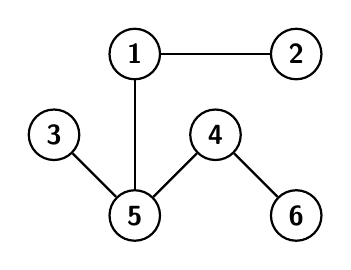
\begin{tikzpicture}[
    node distance=1.45cm, thick,
    main node/.style={circle, draw, font=\sffamily\bfseries}
]
    \node[main node] (1)                    {1};
    \node[main node] (3) [below left  of=1] {3};
    \node[main node] (4) [below right of=1] {4};
    \node[main node] (2) [above right of=4] {2};
    \node[main node] (5) [below right of=3] {5};
    \node[main node] (6) [below right of=4] {6};

    \path (1) edge (2)
        (1) edge (5)
        (3) edge (5)
        (4) edge (5)
        (4) edge (6);
\end{tikzpicture}
\caption{Et tre}
\end{figure}
 \end{column}
 \pause
    \begin{column}{0.48\textwidth}
\begin{figure}
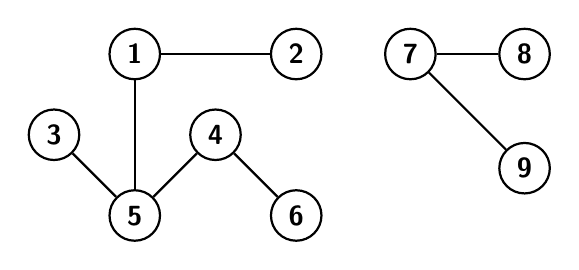
\begin{tikzpicture}[
    node distance=1.45cm, thick,
    main node/.style={circle, draw, font=\sffamily\bfseries}
]
    \node[main node] (1)                    {1};
    \node[main node] (3) [below left  of=1] {3};
    \node[main node] (4) [below right of=1] {4};
    \node[main node] (2) [above right of=4] {2};
    \node[main node] (5) [below right of=3] {5};
    \node[main node] (6) [below right of=4] {6};
    \node[main node] (7) [right of=2] {7};
    \node[main node] (8) [right of=7] {8};
    \node[main node] (9) [below of=8] {9};

    \path (1) edge (2)
        (1) edge (5)
        (3) edge (5)
        (4) edge (5)
        (4) edge (6)
        (7) edge (8)
        (7) edge (9);
\end{tikzpicture}
\caption{En skog}
\end{figure}
\end{column}
\end{columns}
\end{frame}

\begin{frame}{Rotfestede trær}
    \begin{itemize}
        \item Et \emph{rotfestet} tre er et tre med en dedikert rotnode.
        \item Nodene 'under' en annen node kalles for \emph{barnene} til noden.
        \item Noden 'over' en node kalles for forelderen. Alle unntatt roten har en forelder.
        \item Et binærtre er et rotfestet tre der alle har enten 0, 1 eller 2 barn.
    \end{itemize}
    \begin{columns}
    \begin{column}{0.48\textwidth}
\begin{figure}
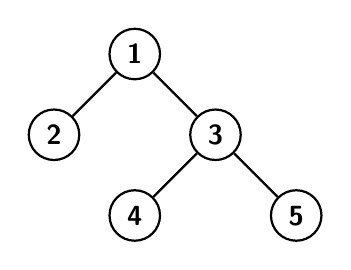
\begin{tikzpicture}[
    node distance=1.45cm, thick,
    main node/.style={circle, draw, font=\sffamily\bfseries}
]
    \node[main node] (1)                    {1};
    \node[main node] (2) [below left  of=1] {2};
    \node[main node] (3) [below right of=1] {3};
    \node[main node] (4) [below left of=3] {4};
    \node[main node] (5) [below right of=3] {5};

    \path (1) edge (2)
        (1) edge (3)
        (3) edge (4)
        (3) edge (5);
\end{tikzpicture}
\caption{binary tre}
\end{figure}
 \end{column}
    \begin{column}{0.48\textwidth}
\begin{figure}
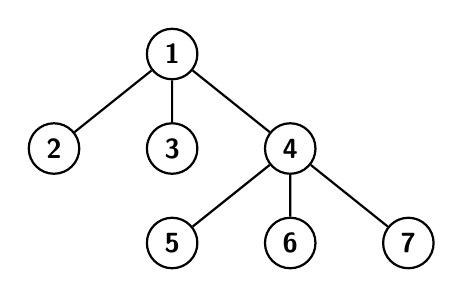
\begin{tikzpicture}[
    node distance=1.45cm, thick,
    main node/.style={circle, draw, font=\sffamily\bfseries},level distance=1.2cm,
  level 1/.style={sibling distance=1.5cm},
  level 2/.style={sibling distance=1.5cm}
]
  \node[main node] {1}
  	child {node[main node] {2}}
    child {node[main node] {3}}
    child {node[main node] {4}
    child {node[main node] {5}}
      child {node[main node] {6}}
    child {node[main node] {7}}
    };
\end{tikzpicture}
\caption{3-ary tre}
\end{figure}
\end{column}
\end{columns}
\end{frame}


\subsection*{Representasjon}
\begin{frame}[fragile]{Måter å oppgi relasjoner på}
    \begin{columns}
        \begin{column}{0.3\textwidth}
            \begin{tikzcd}
            A \arrow[r] \arrow[d] \arrow[rd] & B \arrow[d] \arrow[ld] \\
            D                                & C \arrow[l]           
            \end{tikzcd}
        \end{column}
        \begin{column}{0.65\textwidth}
            \pause
            Kantliste:\\
            $\{(A, B), (A, C), (A, D), (B, C), (B, D), (C, D)\}$\\[5mm]
            \pause
            Settkomprehensjon:\\
            $\{(x, y) | x, y \in \{A,B,C,D\}, x < y\}$:\\[5mm]
            \pause
            \begin{columns}
                \begin{column}{0.27\textwidth}
                    Matrise:\\
                    \begin{math}
                        \begin{matrix}
                              & A & B & C & D\\
                            A & 0 & 1 & 1 & 1\\
                            B & 0 & 0 & 1 & 1\\
                            C & 0 & 0 & 0 & 1\\
                            D & 0 & 0 & 0 & 0
                        \end{matrix}
                    \end{math}
                \end{column}
                \pause
                \begin{column}{0.38\textwidth}
                    Nabolister:\\        
                    $N(A) = [B, C, D]$\\
                    $N(B) = [C, D]$\\
                    $N(C) = [D]$\\
                    $N(D) = []$
                \end{column} 
            \end{columns}
        \end{column}
    \end{columns}
\end{frame}

\begin{frame}[fragile]{Måter å oppgi \sout{relasjoner} grafer på}
    \begin{columns}
        \begin{column}{0.3\textwidth}
            \begin{tikzcd}
            A \arrow[r] \arrow[d] \arrow[rd] & B \arrow[d] \arrow[ld] \\
            D                                & C \arrow[l]           
            \end{tikzcd}
        \end{column}
        \begin{column}{0.65\textwidth}
            \pause
            Kantliste:\\
            $\{(A, B), (A, C), (A, D), (B, C), (B, D), (C, D)\}$\\[5mm]
            \pause
            Settkomprehensjon:\\
            $\{(x, y) | x, y \in \{A,B,C,D\}, x < y\}$:\\[5mm]
            \pause
            \begin{columns}
                \begin{column}{0.27\textwidth}
                    Matrise:\\
                    \begin{math}
                        \begin{matrix}
                              & A & B & C & D\\
                            A & 0 & 1 & 1 & 1\\
                            B & 0 & 0 & 1 & 1\\
                            C & 0 & 0 & 0 & 1\\
                            D & 0 & 0 & 0 & 0
                        \end{matrix}
                    \end{math}
                \end{column}
                \pause
                \begin{column}{0.38\textwidth}
                    Nabolister:\\        
                    $N(A) = [B, C, D]$\\
                    $N(B) = [C, D]$\\
                    $N(C) = [D]$\\
                    $N(D) = []$
                \end{column} 
            \end{columns}
        \end{column}
    \end{columns}
\end{frame}

\subsection{Grafsøk}
\begin{frame}{Søk}
    Om vi har en graf, er det hovedsakelig to måter vi kan søke igjennom grafen: 
    \begin{itemize}
        \item Bredde-Først Søk (BFS)
        \item Dybde-Først Søk (DFS)
    \end{itemize}
    Forskjellen ligger i når hver node blir søkt.
\end{frame}

\begin{frame}[fragile]{BFS}
    Vi holder styr på hvilken 'generasjon' med noder vi jobber med. For hver generasjon ser vi etter alle noder som den generasjonen kan nå, og det er neste generasjon.
    \begin{columns}
        \begin{column}{0.5\textwidth}
            \begin{minted}[fontsize=\scriptsize]{python}
def bfs(start, graph):
    visited = { u: False for u in graph }
    visited[start] = True
    current_gen = [start]
    next_gen = []
    while len(current_gen) > 0:
        for u in current_gen:
            print(u)
            for v in graph[u]:
                if not visited[v]:
                    next_gen.append(v)
                    visited[v] = True
        current_gen, next_gen = next_gen, []
            \end{minted}
        \end{column}
        \begin{column}{0.45\textwidth}
            \begin{figure}
                \centering
                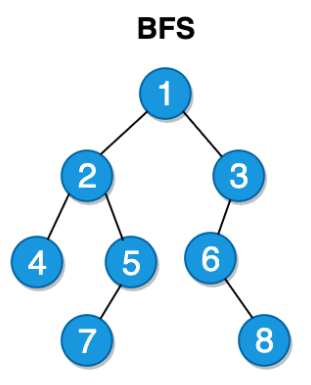
\includegraphics[height=4cm]{images/bfs.png}
                %\caption{Rekkefølgen nodene blir søkt med BFS}
                \label{fig:bfs}
            \end{figure}   
        \end{column}
    \end{columns}
\end{frame}

\begin{frame}[fragile]{DFS}
    Her går vi heller i dybden først. Hver gang vi oppdager en ny node søker vi den umiddelbart før vi går tilbake igjen.
    \begin{columns}
        \begin{column}{0.5\textwidth}
            \begin{minted}[fontsize=\scriptsize]{python}
def dfs(start, graph, visited):
    print(start)
    visited[start] = True
    for v in graph[start]:
        if not visited[v]:
            dfs(v, graph, visited)
            \end{minted}
        \end{column}
        \begin{column}{0.45\textwidth}
            \begin{figure}
                \centering
                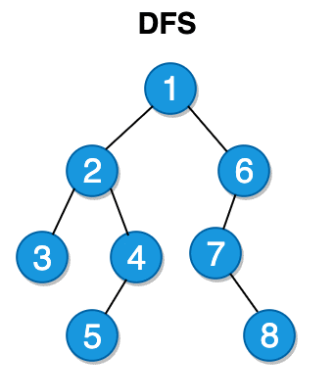
\includegraphics[height=4cm]{images/dfs.png}
                %\caption{Rekkefølgen nodene blir søkt med DFS}
                \label{fig:bfs}
            \end{figure}   
        \end{column}
    \end{columns}
\end{frame}

\subsection{Korteste sti}
\begin{frame}[fragile]{Korteste sti}
    Vi kan bruke BFS til å finne den korteste stien i en graf, og dermed også den korteste ruten til Kvarteret. Men noen kanter/veier tar lengre tid å gå enn andre, så i praksis fungerer det ikke så bra.
    \begin{columns}
        \begin{column}{0.48\textwidth}
            \begin{tikzcd}
            \text{Høytek} \arrow[r] \arrow[d] & B \arrow[r] \arrow[d] & \text{Kvarteret}   \\
            A \arrow[r]                & C \arrow[r]           & D \arrow[u]
            \end{tikzcd}
        \end{column}
        \begin{column}{0.48\textwidth}
            \begin{tikzcd}
            \text{Høytek} \arrow[r, "2"] \arrow[d, "1"] & B \arrow[r, "8"] \arrow[d, "3"] & \text{Kvarteret}        \\
            A \arrow[r, "5"]                     & C \arrow[r, "1"]                & D \arrow[u, "2"]
            \end{tikzcd}
        \end{column}
    \end{columns}
    \begin{definition}[Vektet graf]
        En vektet graf er en der alle kantene også har en vekt/kostnad.
    \end{definition}
\end{frame}

\begin{frame}[fragile]{Dijkstras algoritme}
    Dijkstras algoritme fungerer utmerket for å finne den korteste stien i en vektet graf, så lenge vektene er positive tall.
    \begin{minted}[fontsize=\scriptsize]{python}
def dijkstra(start, end, graph):
    dist = { u: 99999999999999 for u  in graph }
    dist[start] = 0
    queue = [start]
    while len(queue) > 0:
        next = min(queue, key=lambda u: dist[u]) # finner noden med lavest distanse
        queue.remove(next)
        for (v, weight) in graph[next]:
            if dist[v] < dist[next] + weight:
                dist[v] = dist[next] + weight
                queue.append(v)
    return dist
    \end{minted}
\end{frame}

\subsection*{Spørretid}
\begin{frame}{Spørsmål?}
    \begin{figure}
        \centering
        \includegraphics[height = 4.9cm]{images/guillaume9.jpg}
        \caption{Guillaume foran Tvindefossen}
        \label{fig:guillaume9}
    \end{figure}
\end{frame}


%\section*{Slutt}
\begin{frame}
\begin{center}
\begin{Large}
\textbf{Lykke til på eksamen!\\[5mm]
Takk for oss :)}

\end{Large}
\end{center}  
\end{frame}
\end{document}